\documentclass[11pt]{article}

% ---------------------------------------------------------------------------
% HLM5: Certified Knowledge Editing
%   (Closed-form reachability guarantees for additive edits to a frozen LM)
% arXiv-style single-column preprint. Compiles on Overleaf out of the box.
% Figures are vector PDFs under figures/; every quantitative claim traces to a
% measured artifact under results/ in this repository (artifact file names are
% quoted in the table and figure captions).
% ---------------------------------------------------------------------------

\usepackage[margin=1in]{geometry}
\usepackage{amsmath,amssymb,amsthm}
\usepackage{booktabs}
\usepackage{graphicx}
\usepackage{array}
\usepackage{xcolor}
\usepackage[numbers,square]{natbib}
\usepackage[hidelinks]{hyperref}
\usepackage{authblk}

\newtheorem{lemma}{Lemma}
\newtheorem{proposition}{Proposition}
\newtheorem{corollary}{Corollary}
\newtheorem{definition}{Definition}
\theoremstyle{remark}
\newtheorem{observation}{Observation}
\newtheorem{remark}{Remark}
\newtheorem{conjecture}{Conjecture}

\DeclareMathOperator*{\argmax}{arg\,max}
\DeclareMathOperator*{\argmin}{arg\,min}
\DeclareMathOperator{\relu}{relu}
\DeclareMathOperator{\softmax}{softmax}
\DeclareMathOperator{\unit}{unit}
\newcommand{\R}{\mathbb{R}}
\newcommand{\E}{\mathbb{E}}
\newcommand{\Df}{\mathcal{D}_F}
\newcommand{\Dh}{\mathcal{D}_H}
\newcommand{\Dr}{\mathcal{D}_R}

\title{\textbf{Certified Knowledge Editing: Closed-Form Reachability\\
 Guarantees for Additive Edits to a Frozen Language Model}}

\author[1]{Marius Dima}
\affil[1]{Qriton \quad \texttt{marius.dima@qriton.com}}
\date{}

\begin{document}
\maketitle

\begin{abstract}
Knowledge edits to language models are validated only after the fact. We study
the reverse contract: a certificate, computed \emph{before} the edit, of which
edits can succeed. HLM5 attaches a slot memory to a frozen decoder-only
transformer: a hidden-state query selects slots through a hard cosine gate and
adds the value to the pre-head representation. Gate and read see only the
unperturbed hidden state, so logits are affine in the edit strength and
single-token reachability is one-dimensional linear feasibility: a closed-form
certificate, one pass over the head matrix, accepting or refusing each edit in
advance. On a frozen $1$B trunk, $78.4\%$ of $1{,}200$ single-token targets
are reachable at a novel-entity key---$79.4\%\pm2.2\%$ (mean $\pm$ SD) across
$60$ keys---and readout-level residual synthesis rescues $40/40$ sampled
unreachable targets (median $\beta=20$). The certificate also \emph{doses}
each edit: a global strength overshoots the certified interval, silently
failing reachable edits (efficacy $0.529$); the certified $\beta^{\star}$
flips exactly the certificate-reachable set ($0.765$); synthesis rescues the
rest ($1.000$)---at off-support locality $1.000$, zero gradients, paraphrase
transfer $0.020$. A gate-matched static logit bias matches the dosed pipeline
on every measured axis: the value is the a-priori admission test, certified
dose, synthesis rescue, and audit trail, not raw editing power. On $300$
CounterFact records, pre-edit certificate difficulty predicts ROME's
paraphrase transfer ($p<0.01$; fine-tuning directionally, $p=0.02$) and
neighborhood damage for ROME and GRACE ($p<0.01$). Fine-tuning generalizes
only by collapsing locality; HLM5 is a zero-gradient, certificate-gated,
exact-key editor whose every operation emits a verifiable receipt. Full
head-to-head evaluation against MEMIT, MEND, and SERAC on standard benchmarks
remains open.
\end{abstract}

\section{Introduction}

Post-hoc knowledge editing asks how to install a new fact into a trained model so
that the edit (i) takes effect, (ii) does not disturb unrelated behavior, (iii)
can be reversed, and (iv) can be audited. Today these properties are
established, if at all, only \emph{after} the edit is installed; we
instead ask for an \emph{a-priori certificate} that an edit will take and stay local,
and treat a failed certificate as a first-class, audited refusal. Fine-tuning and parameter-efficient
tuning install facts by gradient descent, mixing them into trained parameters so
that locality and reversibility must be re-checked per
edit. Retrieval keeps the trunk fixed but installs knowledge in a prompt-assembly
layer. Locate-and-edit methods such as ROME and MEMIT \citep{meng2022rome,
meng2022memit} mutate trunk weights directly, and deletion is itself another
edit. Wrapper editors such as SERAC and GRACE \citep{mitchell2022serac,
hartvigsen2023grace} instead attach an external, key-addressed store that defers
to the frozen model off-scope.

We place our method, HLM5 (Hopfield Language Model 5), in this last family and ask what becomes provable when
the external read is constrained to a particular form. HLM5 attaches a slot memory
to a frozen decoder-only trunk; a hidden-state query selects slots through a hard
cosine gate, and the selected value is written \emph{additively} into the
pre-head representation at a single position. Because the gate and the read depend
only on the unperturbed hidden state, the perturbed logits are affine in the
scalar edit strength $\beta$. Reachability of a single-token target then reduces
to one-dimensional linear feasibility, which we solve in closed form. The result
is a certificate---computable before injection---that labels each target as
reachable or unreachable under the deployed configuration. Editing becomes an
admission test with an a-priori guarantee, not a gradient step whose locality is
audited after the fact.

HLM5 is also the certified fragment of a broader ``energy language'' program that
treats memory slots as attractor basins to be surveyed, injected, strengthened,
forgotten, and transplanted rather than retrained~\citep{qriton2026energylang,
qriton2026hlm}; we consolidate that correspondence, and operational checks of the
operator set on a real co-trained memory, in Section~\ref{sec:energyops}.

\paragraph{Contributions.}
\begin{enumerate}
  \item \textbf{A reachability certificate (Section~\ref{sec:theory}).} Because
  the post-edit logit margins are affine in the edit strength
  (Lemma~\ref{lem:affine}), we give a closed-form test
  (Proposition~\ref{prop:reach}) for whether a finite edit strength makes a
  target win, and a corollary (Corollary~\ref{cor:unflip}) that certifies
  unreachable targets a priori. On the frozen $1$B trunk the certificate yields
  a full operating envelope---$259$ of $1{,}200$ targets certified unreachable in
  advance at the reference key, stable at $79.4\%\pm2.2\%$ reachable across $60$
  diverse keys---and residual synthesis rescues all $40$ sampled unreachable
  targets in a readout-level verification (Section~\ref{sec:envelope}).
  \item \textbf{A zero-tax co-training result (Section~\ref{sec:notax}).} Under a
  matched-pair protocol, adding the memory module changes validation perplexity by
  $+0.018\%$ at $136$M and $-0.116\%$ at $1$B.
  \item \textbf{A governed update contract (Sections~\ref{sec:setup}--\ref{sec:results}).}
  Injection, tamper-evident receipts, edit, forget, and an exact off-support
  fallback are evaluated as first-class behaviors, with measured boundaries
  reported alongside the successes.
\end{enumerate}

The scope is deliberately narrow. Edits are single-token and
exact-key; paraphrase transfer is weak; the additive read degrades multi-query
in-context recall; the capacity studies are synthetic; numbers are single-seed;
and head-to-head baselines on standard editing benchmarks are not yet run. We
state each as a limitation with an explicit pass/fail experiment
(Section~\ref{sec:limits}).

\section{Related Work}
\label{sec:related}

We compare methods by update contract rather than by model family.
\emph{Fine-tuning and PEFT}---continued training, LoRA \citep{hu2021lora}, prefix
tuning \citep{li2021prefix}, constrained fine-tuning \citep{zhu2020modifying}---install
facts by optimization. \emph{Retrieval} \citep{lewis2020rag} conditions a frozen
generator on retrieved passages, and in-context editing \citep{zheng2023ike}
installs the counterfactual directly in the prompt. \emph{Datastore memory},
kNN-LM and RETRO
\citep{khandelwal2019knnlm, borgeaud2021retro}, interpolates the output
distribution with a nearest-neighbor distribution over a key--value store.
\emph{Locate-and-edit} methods---knowledge neurons \citep{dai2022neurons}, ROME
and MEMIT \citep{meng2022rome, meng2022memit}, and their successors PMET
\citep{li2024pmet} and AlphaEdit \citep{fang2025alphaedit}---solve a constrained
update to feed-forward projections, although the localization premise itself has
been questioned \citep{hase2023localization}.
\emph{Wrapper and meta-learned editors}---KnowledgeEditor \citep{decao2021editing},
MEND \citep{mitchell2021mend}, SERAC \citep{mitchell2022serac}, CaliNet
\citep{dong2022calinet}, T-Patcher \citep{huang2023tpatcher}, GRACE
\citep{hartvigsen2023grace}, MELO \citep{yu2024melo}, WISE \citep{wang2024wise},
Larimar \citep{das2024larimar}, and MEMOIR \citep{wang2025memoir}---wrap the
frozen trunk with an external cache, codebook, side memory, or hypernetwork.
Surveys and benchmarks \citep{yao2023editing, zhang2024knowedit} and toolkits
\citep{wang2023easyedit} standardize the evaluation around reliability,
generalization, locality, and portability \citep{zhong2023mquake} on CounterFact
\citep{meng2022rome} and zsRE \citep{levy2017zeroshot}. A parallel line documents
what editing costs: ripple effects on logically related facts
\citep{cohen2024ripple}, knowledge distortion \citep{li2024pitfalls}, degradation
of general abilities \citep{gu2024harms}, and gradual or even catastrophic
collapse under sequential weight edits \citep{gupta2024forgetting,
yang2024butterfly}---failure modes that motivate keeping the trunk frozen and the
edits external, as here.

\emph{Representation-space editing and steering.} Closest in mechanism to our
additive pre-head write are methods that edit \emph{activations} rather than
weights: REMEDI learns fact encodings added to hidden representations
\citep{hernandez2024remedi}, activation addition steers generation with
difference vectors \citep{turner2023actadd}, inference-time intervention shifts
attention-head outputs along learned directions \citep{li2023iti}, and
representation engineering generalizes the recipe \citep{zou2023repe}; the
reliability of such steering vectors in and out of distribution is itself under
scrutiny \citep{tan2024steering}. The additive hidden-state write is therefore
established prior art. What none of these provide---and what the specific
combination of a hard support gate with a write at the \emph{pre-head} position
makes possible---is a \emph{closed-form, a-priori reachability certificate}:
because our gate and read depend only on the unperturbed hidden state, every
logit margin is affine in the edit strength, and admission or refusal of an edit
is decidable before it is applied (Section~\ref{sec:theory}).

\emph{Associative memory and modern Hopfield networks.} Classical Hopfield networks
store patterns as attractors of an energy landscape \citep{hopfield1982neural};
Dense Associative Memory raises storage capacity by sharpening the interaction to a
high-order polynomial \citep{krotov2016dense, krotov2021large}, its continuous,
softmax form underlies modern Hopfield layers \citep{ramsauer2020hopfield}, and
engineered energy functions have since been built into transformer blocks
themselves \citep{hoover2023energy}; see \citet{krotov2025modern} for a current
treatment. HLM5's
gate (\S\ref{sec:method}) is exactly such a degree-$\kappa$ associative read, but
attached \emph{externally} and coupled \emph{additively} to a frozen trunk rather
than realized as the network's own dynamics---which is what makes each edit
certifiable (\S\ref{sec:theory}).

HLM5 belongs to the wrapper-editor family: GRACE already maintains a
key-addressed codebook that defers to the frozen trunk off-scope, and SERAC
routes in-scope queries to a counterfactual store. HLM5 claims no novelty for
the wrapper architecture itself, nor for the additive activation write
(REMEDI, ActAdd, ITI above). Its specific, analyzable choice is an \emph{additive}
pre-head read with a hard cosine gate, which makes the logits affine in the edit
strength and therefore admits the closed-form reachability certificate of
Section~\ref{sec:theory}---to our knowledge the first a-priori admission test
with refusal receipts in the editing literature. We position HLM5 within this
family and treat the head-to-head benchmark comparison as the primary open
evaluation (E1, Section~\ref{sec:limits}).

\section{Problem Statement and Preliminaries}
\label{sec:prelim}

\paragraph{Notation.}
Let $f_\theta$ be a decoder-only language model with parameters $\theta$ mapping a
prefix $x=(x_1,\dots,x_t)$ to a final hidden state $h=f_\theta(x)\in\R^{d}$ and,
through a tied head $W\in\R^{|V|\times d}$, to logits $z=Wh$ and a distribution
$p_\theta(\cdot\mid x)=\softmax(Wh)$. Vectors are columns in inner products;
$W_y\in\R^{d}$ denotes the $y$-th row of $W$; $\unit(x)=x/\lVert x\rVert_2$;
hidden states act as row vectors where the whitening map $A$ multiplies on the
right. A \emph{fact} is a key--target pair $(x,y)$
with a single target token $y\in V$. We restrict targets to one token throughout;
multi-token targets---sequences of such installs, at the cost of the per-step
guarantees below---are deferred to future work (E4,
Section~\ref{sec:limits})~\citep{jiang2025anyedit}. We write $\Df$ for the facts to install and
$\Dh$ for held-out text, the latter taken disjoint from the support of installed
keys.

\paragraph{Problem.} Given a trunk trained once and facts $\Df$ arriving
afterward, install each $(x,y)$ so that (i)~\emph{efficacy}:
$\argmax_{y'\in V} p_{\theta'}(y'\mid x)=y$; (ii)~\emph{locality}: behavior on
$\Dh$ is preserved; (iii)~\emph{reversibility}: an installed fact can be edited or
deleted; (iv)~\emph{auditability}: every operation emits a verifiable receipt.
Criteria (i)--(ii) are the editing literature's reliability and
locality/specificity; \emph{generalization} (survival under paraphrases) is out
of scope by construction and measured empirically (Section~\ref{sec:gen}).

We state the existing families as objectives over $(x,y)\in\Df$. Supervised
fine-tuning installs the fact by
\begin{equation}
\mathcal{L}_{\mathrm{FT}}(\theta)=\E_{(x,y)\sim\Df}\!\left[-\log p_\theta(y\mid x)\right],
\end{equation}
spreading the update across all of $\theta$. LoRA restricts the write to a
low-rank delta on a frozen internal weight $W_0\in\R^{d\times k}$ (any projection
other than the head $W$),
\begin{equation}
W_0' = W_0 + \tfrac{\alpha}{r}\,BA,\quad B\in\R^{d\times r},\ A\in\R^{r\times k},\ r\ll\min(d,k).
\end{equation}
Retrieval-augmented generation marginalizes over retrieved passages $c$ with the
trunk fixed and the corpus $\Dr$ as the editable memory,
\begin{equation}
p(y\mid x)=\sum_{c\in R_\eta(x)} p_\eta(c\mid x)\, p_\theta(y\mid x,c),
\end{equation}
the RAG-Sequence form of \citet{lewis2020rag}. kNN-LM interpolates the output with
a datastore distribution under a global weight $\lambda$,
\begin{equation}
p(y\mid x)=\lambda\, p_{k\mathrm{NN}}(y\mid x)+(1-\lambda)\,p_\theta(y\mid x).
\end{equation}
ROME edits a feed-forward down-projection $W_\ell$, viewed as a linear
associative memory, by the rank-one update that installs $(k_*,v_*)$ while
least-squares preserving prior associations with uncentered key covariance
$C=\E[kk^{\top}]$,
\begin{equation}
\widehat{W}_\ell = W_\ell + \frac{(v_*-W_\ell k_*)\,(C^{-1}k_*)^{\top}}{(C^{-1}k_*)^{\top}k_*}.
\end{equation}
Across these, the update mutates either trunk parameters (fine-tuning, LoRA,
ROME/MEMIT) or input context (RAG, prefix-tuning), and locality, reversibility,
and deletion must be established after the fact. HLM5 instead fixes $\theta$ and installs each fact as
an entry in an external gated memory (Section~\ref{sec:method}).

\section{Method}
\label{sec:method}

\paragraph{Frozen trunk.} The trunk is a standard decoder-only transformer with
tied embedding and head. The $1$B configuration uses width $1792$, $24$ layers,
$14$ heads, sequence length $1024$, and vocabulary $65{,}536$. We use the memory
in two distinct ways and keep them separate throughout: the \emph{hybrid arm}
co-trains the memory module during pretraining (the no-tax study,
Section~\ref{sec:notax}); the \emph{injection protocol} attaches an editable
memory to the \emph{frozen baseline} trunk at inference (the edit/forget study,
Section~\ref{sec:spread}). Figure~\ref{fig:pipeline} contrasts the two.

\begin{figure}[t]
\centering
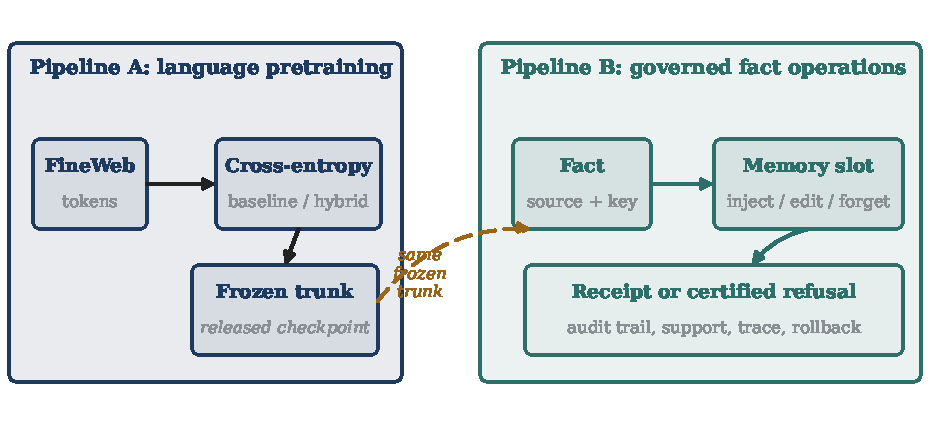
\includegraphics[width=0.95\linewidth]{figures/fig1-pipeline-a-b.pdf}
\caption{Two pipelines. Pipeline~A pretrains the trunk once (optionally
co-training the memory module); Pipeline~B governs fact create/edit/forget on the
\emph{same} frozen trunk, with receipts. Pipeline~B never retrains the
Pipeline~A trunk; no per-fact gradient.}
\label{fig:pipeline}
\end{figure}

\paragraph{Editable memory.} The memory holds slots
$s_i=(k_i,v_i,\alpha_i,\text{label}_i,\text{active}_i)$. From a hidden state $h$
the query is mean-centered and optionally whitened to counter the anisotropy of
trained hidden states \citep{ethayarajh2019contextual, gao2019degeneration},
\begin{equation}
q=(h-\mu)A,
\end{equation}
with $\mu$ the mean hidden state over a calibration set of fact-key and neutral
prompts and $A$ identity or a ZCA whitening matrix estimated from the same
calibration set; both are frozen at audit time. With $q$ and
keys unit-normalized, slot $i$ scores through a degree-$\kappa$ cosine kernel---a
Dense Associative Memory interaction of polynomial order~\citep{krotov2016dense}---gated
by an active flag and a nonnegative strength,
\begin{equation}
s_i(q)=\text{active}_i\cdot\relu(\alpha_i)\cdot\max\!\big(0,\cos(q,k_i)\big)^{\kappa},\qquad \kappa=5,
\label{eq:score}
\end{equation}
and the read is a temperature-softmax mixture of values,
\begin{equation}
r(q)=\softmax\!\big(s(q)/T\big)\,V,\qquad T=0.1.
\end{equation}
The memory perturbs the pre-head representation---after the trunk's final layer
normalization, immediately before the bias-free tied head---and only when the
maximum score crosses a hard support threshold $\tau$:
\begin{equation}
g(q)=\begin{cases}\max_i s_i(q) & \max_i s_i(q)\ge\tau\\ 0 & \text{otherwise,}\end{cases}
\qquad h'=h+\beta\,g(q)\,r(q),\quad z'=Wh',
\label{eq:hook}
\end{equation}
with $\tau=0.95$ and edit-strength scalar $\beta$. We write
$\beta_{\mathrm{eff}}=\beta\,g(q)$ and $\bar r=r(q)$ for the realized residual.
Figure~\ref{fig:arch} shows the full forward pass.

\paragraph{Value construction.} For single-token injection the slot value is the
unit output embedding of the target,
\begin{equation}
v=\unit(W_y).
\end{equation}
A target $y$ is \emph{head-reachable} if its embedding row is its own nearest
neighbor in the tied head, $\argmax_{j}(WW_y)_j=y$; at $1$B, $10.27\%$ of the
vocabulary is head-reachable. A head-geometry audit shows this is a property of
the output head, not of the memory: reachability varies sharply with embedding
norm (Figure~\ref{fig:headgeom})---from $30.7\%$ in the lowest-norm decile to
$2.7$--$6.7\%$
in the middle deciles---unreachable tokens have a median self-nearest-neighbor rank of $6{,}472$, and their
confusers are dominated by high-frequency tokens and punctuation (e.g.\ ``\,that''
and ``\,with'', shown with their leading space, are outranked by ``,''). This is
the ``stolen-probability'' effect \citep{demeter2020stolen} produced by the
anisotropic, narrow-cone geometry of tied output embeddings
\citep{gao2019degeneration, ethayarajh2019contextual} and bounded ultimately by
the rank of the softmax head \citep{yang2018bottleneck}. Many edit failures are
therefore head-geometry failures rather than memory
failures. Head-reachability is necessary but not sufficient for an edit at a given
$h$; sufficiency is the $\beta$-feasibility test of Section~\ref{sec:theory}.

\begin{figure}[t]
\centering
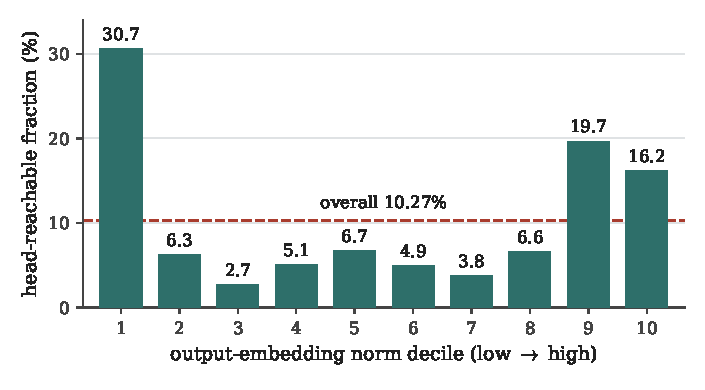
\includegraphics[width=0.72\linewidth]{figures/fig-head-geometry.pdf}
\caption{Head-reachability is a property of the output head, not the memory. The
head-reachable fraction of the vocabulary varies sharply across output-embedding
norm deciles ($30.7\%$ in the lowest decile, $2.7$--$6.7\%$ in the middle, rising
again at high norm), around an overall $10.27\%$; unreachable tokens sit a median
of $6{,}472$ ranks from their own nearest neighbor. Measured on the frozen $1$B
trunk (\texttt{headgeom\_metrics.json}).}
\label{fig:headgeom}
\end{figure}

\begin{figure}[t]
\centering
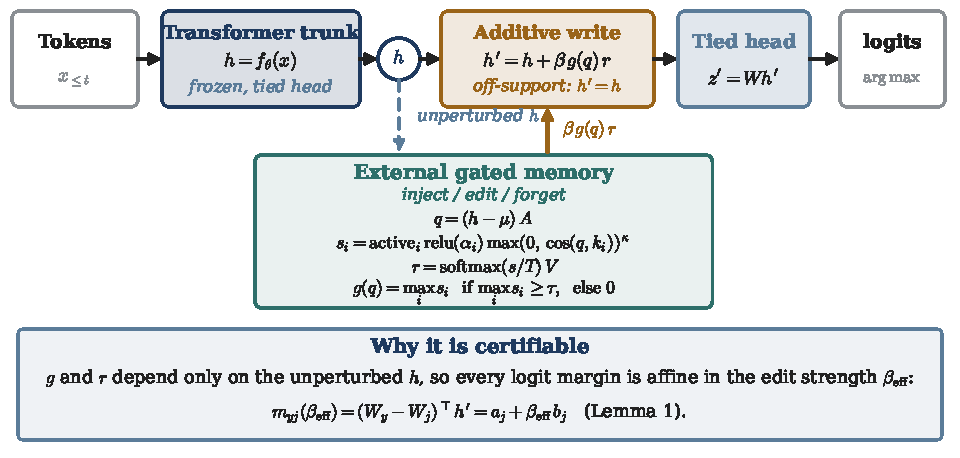
\includegraphics[width=0.98\linewidth]{figures/fig-arch-forward.pdf}
\caption{HLM5 forward pass. The frozen trunk produces the hidden state $h$; a
mean-centered, whitened query $q=(h-\mu)A$ scores slots with a degree-$\kappa$ cosine
kernel, and a hard support gate either writes the boosted value $\beta\,g(q)\,r$
additively into the pre-head state or leaves the trunk untouched. Because the query,
gate, and read all read the \emph{unperturbed} $h$, every logit margin is affine in
the edit strength (Lemma~\ref{lem:affine})---the property the certificate rests on.}
\label{fig:arch}
\end{figure}

\section{Reachability and Off-Support Fallback}
\label{sec:theory}

All statements below concern a single decoded position with $h$ the unperturbed
hidden state, $\bar r=r(q)$ the realized residual, and $\beta_{\mathrm{eff}}\ge 0$.
The write modifies only the readout at that position---it enters neither the
residual stream nor the attention state---so within a forward pass it cannot
affect other positions' hidden states; under generation, later positions are
affected only through the emitted token, and each per-position guarantee is
conditional on its realized prefix. Feasibility is stated in
$\beta_{\mathrm{eff}}=\beta\,g(q)$; it transfers to the deployed dial $\beta$
exactly when the gate fires at the key ($g(q)\ge\tau>0$), which the measured gate
selectivity guarantees at exact keys (\S\ref{sec:envelope}).

\begin{lemma}[Margins are affine in edit strength]
\label{lem:affine}
The gate $g(q)$ and read $\bar r$ depend only on $q$, which is a function of the
unperturbed $h$. Hence, for any competitor $j$, the post-edit margin of target
$y$ is affine in $\beta_{\mathrm{eff}}$:
\[
m_{yj}(\beta_{\mathrm{eff}}) = (W_y-W_j)^{\top}h' = a_j + \beta_{\mathrm{eff}}\,b_j,
\quad a_j=(W_y-W_j)^{\top}h,\ \ b_j=(W_y-W_j)^{\top}\bar r .
\]
\end{lemma}
\begin{proof}
By \eqref{eq:hook}, $h'=h+\beta_{\mathrm{eff}}\bar r$ with $\bar r$ and the gate
constant in $\beta_{\mathrm{eff}}$ since they are determined by $q=(h-\mu)A$.
Substituting and using linearity of $(W_y-W_j)^{\top}(\cdot)$ gives the stated
affine form.
\end{proof}

\begin{proposition}[$\beta$-feasibility]
\label{prop:reach}
Target $y$ wins against all competitors (strictly: $m_{yj}>0$ for all $j\ne y$)
for some finite
$\beta_{\mathrm{eff}}\ge 0$ if and only if
\[
\begin{aligned}
&\big(\forall j:\ b_j=0 \Rightarrow a_j>0\big)\quad\text{and}\\
&\max\!\Big(0,\ \max_{j:\,b_j>0}\tfrac{-a_j}{b_j}\Big)
\;<\;
\min_{j:\,b_j<0}\tfrac{-a_j}{b_j},
\end{aligned}
\]
where the right-hand side is $+\infty$ when no competitor has $b_j<0$.
\end{proposition}
\begin{proof}
By Lemma~\ref{lem:affine} a strict win requires $m_{yj}(\beta_{\mathrm{eff}})>0$
for every $j\ne y$, i.e.\ $a_j+\beta_{\mathrm{eff}}b_j>0$. This is one-dimensional
linear feasibility in $\beta_{\mathrm{eff}}\ge 0$. If $b_j=0$ the constraint is
$a_j>0$, independent of $\beta_{\mathrm{eff}}$. If $b_j>0$ it gives the lower bound
$\beta_{\mathrm{eff}}>-a_j/b_j$; if $b_j<0$ it gives the upper bound
$\beta_{\mathrm{eff}}<-a_j/b_j$. The feasible set is the intersection
$(L,U)\cap[0,\infty)$ with $L=\max(0,\max_{b_j>0}(-a_j/b_j))$ and
$U=\min_{b_j<0}(-a_j/b_j)$, which is nonempty iff $L<U$ and all $b_j=0$
constraints hold.
\end{proof}
\noindent The feasible set is open at $L$: at $\beta_{\mathrm{eff}}=L>0$ the
binding blocker ties rather than loses. The endpoint $\beta_{\mathrm{eff}}=0$ is
feasible iff $y$ already wins un-edited (all $a_j>0$), in which case $L=0$. We
write the interval as $(L,U)$ throughout.

\begin{corollary}[Unreachability certificate]
\label{cor:unflip}
If some competitor $j$ has $a_j\le 0$ and $b_j\le 0$, then no finite
$\beta_{\mathrm{eff}}\ge 0$ makes $y$ win: $y$ is certified unreachable under this
value direction and gate. The certificate is computable from $h$, $W$, and
$\bar r$ before any injection.
\end{corollary}
\noindent Corollary~\ref{cor:unflip} is sufficient, not exhaustive: a target is
also unreachable when the interval is empty ($L\ge U$) with no single hard
blocker. In the $1$B operating envelope (\S\ref{sec:envelope}), $229$ of the
$259$ certified-unreachable targets at the reference key trip the hard-blocker
clause and the remaining $30$ are refused by an empty interval. For example the target
token ``\,that'' is blocked by the high-frequency competitor ``,'': under the deployed
value $v=\unit(W_y)$ its worst-case competitor margin is negative ($-0.055$) with
non-positive slope, so no finite $\beta_{\mathrm{eff}}\ge0$ flips it and the certificate
refuses it in advance---while residual synthesis (\S\ref{sec:synth}) restores a positive
margin ($+0.42$) and rescues it (Figure~\ref{fig:reach}).

\begin{figure}[t]
\centering
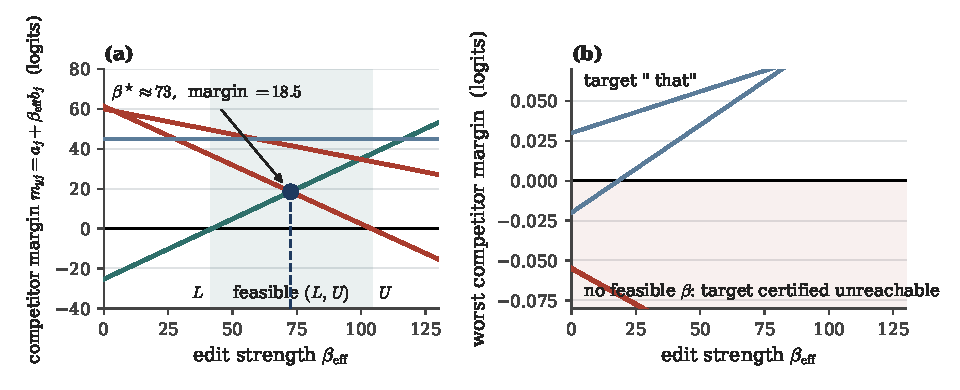
\includegraphics[width=0.98\linewidth]{figures/fig-reachability-geometry.pdf}
\caption{The certificate is one-dimensional linear feasibility
(Proposition~\ref{prop:reach}, Corollary~\ref{cor:unflip}). Each line is a competitor
margin $m_{yj}(\beta_{\mathrm{eff}})=a_j+\beta_{\mathrm{eff}}b_j$; the target wins where
all lie above zero. \textbf{(a)}~A reachable target: the feasible interval $(L,U)$ is
non-empty and $\beta^{\star}$ maximizes the worst-case margin (values from
\texttt{betastar.json}). \textbf{(b)}~An unreachable target (``\,that'', blocked by
``,''): a competitor with $a_j\le0,\ b_j\le0$ stays below zero for every
$\beta_{\mathrm{eff}}$, so the certificate refuses it before injection. Representative
competitor lines drawn to scale around the measured operating point.}
\label{fig:reach}
\end{figure}

\begin{observation}[Forget]
\label{obs:forget}
Setting $\text{active}_i=0$ removes slot $i$'s contribution from $s(\cdot)$ at
every future query, so the post-forget behavior equals that of the memory with
slot $i$ absent, while a tombstone record persists in the audit log.
\end{observation}

\begin{lemma}[Off-support fallback, by construction]
\label{lem:offsupport}
At any position where $\max_i s_i(q)<\tau$, \eqref{eq:hook} gives $g(q)=0$, hence
$h'=h$ and $z'=z$: the distribution is identical to the frozen trunk.
\end{lemma}
\noindent This is an immediate consequence of the hard gate rather than a deep
result; we state it to make the fallback explicit. Whole-sequence locality on
$\Dh$ follows \emph{only if} no held-out query enters the support region
$S_\tau=\{q:\max_i s_i(q)\ge\tau\}$. We do not prove this; we \emph{measure} it
(zero off-support changes, Section~\ref{sec:spread}), and distinguish the
per-position by-construction fact (Lemma~\ref{lem:offsupport}) from the measured
whole-sequence locality.

\begin{conjecture}[Multi-slot rescue]
\label{conj:multi}
The realized residual $\bar r=r(q)$ is a single query-fixed softmax point, not a
free convex combination of slot values. We conjecture that a slot bundle whose
fixed mixture realizes a direction with $b_j>0$ against every blocking competitor
can render an otherwise-unreachable target reachable; establishing the achievable
residual set is left to future work.
\end{conjecture}

\section{Experimental Setup}
\label{sec:setup}

\paragraph{Protocol.} Each scale uses matched-pair pretraining: the baseline and
hybrid arms share data, tokenizer, horizon, optimizer, and seed, differing only in
the hybrid arm's co-trained memory module. Trunks are trained on FineWeb-derived
tokens \citep{penedo2024fineweb}; the tokenizer is a $65{,}536$-symbol BPE
trained on the same distribution, and FineWeb is released under ODC-By~1.0. The
$1$B run uses width $1792$/$24$L/$14$H,
sequence length $1024$, AdamW (betas $0.9,0.95$, base LR $2\!\times\!10^{-4}$,
$2000$-step warmup, cosine decay), gradient clip $1.0$, weight decay $0.1$, and a
single fixed seed. Injection studies attach the editable memory to the frozen
baseline checkpoint; no gradient steps are taken for any fact. The $17$-fact
set used throughout the deployed $1$B studies is listed in
Table~\ref{app:facts} (Appendix).

\paragraph{Compute.} Pretraining ran on the Leonardo Booster GPU partition
(CINECA; $4\times$A100-64GB nodes) under a EuroHPC AI Factory allocation, in
bf16 with periodic validation
and checkpointing; each $1$B arm trained for $153{,}000$ steps at effective
batch $128\times1024$ tokens ($\approx20$B
tokens per arm; \texttt{baseline\_train\_summary.json},
\texttt{hybrid\_train\_summary.json}). The released $1$B checkpoints are the
best-validation snapshots within that schedule---step $150{,}999$ (baseline) and
step $149{,}999$ (hybrid; \texttt{notax\_params.json}). The certificate,
envelope, and editing studies ran on a single RTX~4000~Ada (20\,GB)
workstation.

\paragraph{Metrics.} We adopt the editing literature's axes and give the
correspondence to our measured quantities in Table~\ref{tab:crosswalk}.
Off-support locality is measured as argmax preservation on held-out prompts:
$8$ neutral prompts per fact at $1$B ($136$ prompt--fact checks over $17$ facts)
and the other facts' key prompts ($23$ per fact) in the GPT-2 study. All
reported numbers are single-seed; sampling uncertainty over facts is reported as
bootstrap $95\%$ confidence intervals ($2{,}000$ resamples) in
Tables~\ref{tab:main}, \ref{tab:gpt2}, and~\ref{tab:trunk}, with printed
interval endpoints rounded outward to two decimals, while seed-to-seed
variance is deferred to E6 (Section~\ref{sec:limits}).

\begin{table}[t]
\centering
\small
\begin{tabular}{@{}l l >{\raggedright\arraybackslash}p{0.49\linewidth}@{}}
\toprule
Canonical axis & Our quantity & Definition \\
\midrule
Efficacy / reliability & flip rate & fraction of $K$ facts whose post-edit argmax is the target \\
Generalization & paraphrase rate & fraction of paraphrases of $x$ that yield the target \\
Locality (off-support) & holdout changes & argmax changes on held-out text between detached/attached memory \\
Locality (on-support) & \emph{(pending)} & neighborhood specificity; not yet measured (Section~\ref{sec:limits}) \\
Reversibility & edit/forget + others-intact & edit flips to a new target; forget reverts; others preserved \\
Cost & gradient steps & optimization steps required per fact ($0$ for HLM5) \\
Auditability & receipt & replay-verifiable, tamper-evident record per operation \\
\bottomrule
\end{tabular}
\caption{Crosswalk between the standard editing axes and the quantities measured
here. ``On-support'' neighborhood specificity is a recognized locality test we do
not yet run; ``holdout changes'' measures only off-support locality.}
\label{tab:crosswalk}
\end{table}

\section{From Certificate to Operating Envelope}
\label{sec:envelope}

\paragraph{The operating envelope, not a binary verdict.}
Section~\ref{sec:theory} certifies a target as reachable or not; for deployment we
report the full feasible interval and a risk label. Throughout this section we
work at the exact key, where the measured gate score is $1.00$ (so
$\beta_{\mathrm{eff}}=\beta$; Figure~\ref{fig:gate}) and the temperature-softmax
read concentrates on the injected slot (measured own-slot weight $0.9993$ at
$T=0.1$, $K=17$; \texttt{ownslot\_weight\_certdosed.json}), so
slopes are computed directly against the slot value: the certificate is exact in
$(\beta_{\mathrm{eff}},\bar r)$ and inherits at most this concentration error
here. With the deployed value
$v=\unit(W_y)$ and slope $b_j=(W_y-W_j)^{\top}v$, the feasible edit strengths form
$(L,U)$ with $L=\max(0,\max_{b_j>0}-a_j/b_j)$ and $U=\min_{b_j<0}-a_j/b_j$. To each
edit we attach the interval $(L,U)$, the chosen $\beta$, the slack $U-L$, the
binding blocker token, and a label: \emph{safe} (wide slack), \emph{narrow},
\emph{brittle} (small slack), or \emph{unreachable} ($L\ge U$, or a competitor with
$a_j\le0,\ b_j\le0$). Measured on the frozen $1$B trunk over $1{,}200$ word-like
single-token targets---leading-space single tokens whose text is purely
alphabetic with at least three letters; the first $1{,}200$ such token ids---at
a novel-entity key (Table~\ref{tab:envelope}), $78.4\%$ are
reachable ($74.0\%$ safe) and $21.6\%$ unreachable, with median reachable slack
$30.2$. The envelope is computed before any injection, from $W$ and $h$ in one
pass over the head matrix---a practical admission test, not only a theorem.

\paragraph{Stability across keys.}
The reference-key envelope is not an artifact of one hidden state. Repeating the
computation with the same $1{,}200$-target pool over $60$ diverse key
contexts---$20$ novel-entity templates across several relations, $20$ real-entity
factual prompts, and $20$ generic sentence prefixes---the reachable fraction is
$79.4\%\pm2.2\%$ (min $74.2\%$, max $85.0\%$); a Kruskal--Wallis test finds the
three prompt categories statistically indistinguishable ($H=0.31$, $p=0.86$;
\texttt{multikey\_\allowbreak category\_\allowbreak test.json}). The reference
key ($78.4\%$) sits at the $33$rd percentile (Figure~\ref{fig:envmultikey}). Per key, a mean of $205$
refusals trip the hard-blocker clause of Corollary~\ref{cor:unflip} and $42$ have
an empty interval.

\begin{figure}[t]
\centering
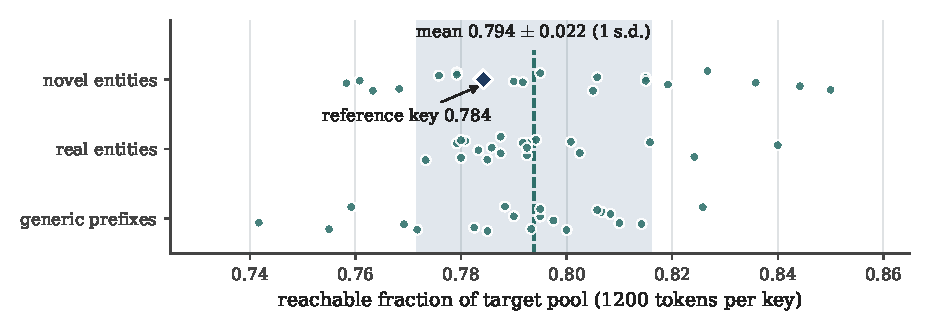
\includegraphics[width=0.95\linewidth]{figures/fig-envelope-multikey.pdf}
\caption{The operating envelope is stable across key contexts. Reachable
fraction of the fixed $1{,}200$-token target pool for $60$ diverse keys ($20$
novel-entity, $20$ real-entity, $20$ generic sentence prefixes): mean
$79.4\%\pm2.2\%$ (shaded); the reference key of Table~\ref{tab:envelope}
($78.4\%$) is typical. Data: \texttt{cert\_envelope\_multikey.json}.}
\label{fig:envmultikey}
\end{figure}

\begin{table}[t]
\centering\small
\begin{tabular}{l r r}
\toprule
Risk label & Count & Fraction \\
\midrule
Safe & $888$ & $74.0\%$ \\
Narrow & $38$ & $3.2\%$ \\
Brittle & $15$ & $1.25\%$ \\
Unreachable & $259$ & $21.6\%$ \\
\bottomrule
\end{tabular}
\caption{Operating-envelope certificate over $1{,}200$ word-like single-token
targets at a novel-entity key on the frozen $1$B trunk, deployed value
$v=\unit(W_y)$. Median reachable slack $U-L=30.2$, computed pre-injection from $W$
and $h$. Residual synthesis (\S\ref{sec:synth}) rescues $40/40$ sampled unreachable
targets.}
\label{tab:envelope}
\end{table}

\paragraph{Choosing the deployment strength.}
Rather than a heuristic value we select the strength that maximizes the
worst-case competitor margin,
\[
\beta^{\star}=\argmax_{\beta\in(L,\,\min(U,\beta_{\max})]}\ \min_{j\ne y}\,(a_j+\beta b_j),
\]
with an explicit cap $\beta_{\max}$ for the case $U=\infty$. The inner objective is concave
and piecewise-linear in $\beta$; we approximate the maximizer on a dense grid
over the capped interval (exact scanning of the breakpoints is equally cheap).
On the $1$B trunk this lifts the median worst-case margin from $1.08$
under the heuristic $\beta=1.05L+1$ to $18.39$ at $\beta^{\star}\approx72$---a
$\approx17\times$ improvement, or a $+17.31$ logit-margin delta, at identical compute
(Figure~\ref{fig:betastar}). The receipt records
$\beta^{\star}$, the slack $U-L$, the active blocker
$j^{\star}=\argmin_{j}(a_j+\beta^{\star}b_j)$, and the realized margin
$M(\beta^{\star})$. Dosing is not cosmetic: on the deployed $17$-fact set a
global strength of $102.8$ exceeds $U$ for four \emph{reachable} facts and
silently fails them (efficacy $0.529$), while dosing at $\beta^{\star}$ flips
all $13$ certificate-reachable facts---efficacy equal to the reachable fraction
exactly---at bit-identical off-support locality (\S\ref{sec:controlled},
\texttt{hlm5\_1b\_faithful\_certdosed.json}).

\begin{figure}[t]
\centering
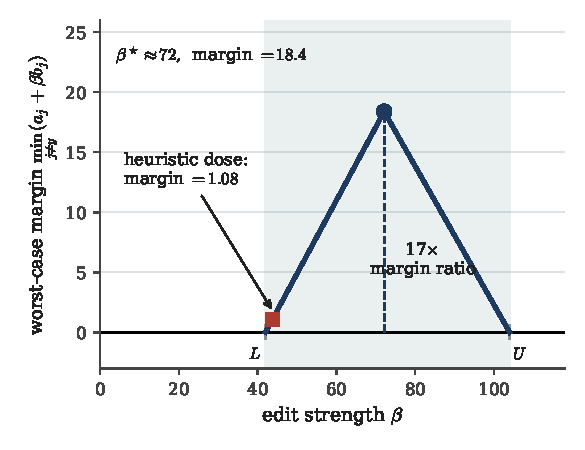
\includegraphics[width=0.6\linewidth]{figures/fig-betastar.pdf}
\caption{Selecting the deployment strength. The tent is a \emph{representative
median envelope} over the $941$-fact reachable set, not any single fact's
trajectory: the worst-case competitor margin $\min_{j\ne y}(a_j+\beta b_j)$ is
concave and piecewise-linear in $\beta$, with $\beta^{\star}$ at its peak. The
peak ($\beta^{\star}\approx72$, worst-case margin $18.39$) and the heuristic
margin ($1.08$ at $\beta=1.05L+1$, giving the $\approx17\times$ ratio and
$+17.31$ logit-margin delta) are
\emph{per-fact medians} over that set (\texttt{betastar.json}). The feasible-band
edges $L,U$ are representative anchors shared with Figure~\ref{fig:reach}, not a
measured $(L,U)$ for any one fact.}
\label{fig:betastar}
\end{figure}

\paragraph{A robust certificate under hidden-state drift.}
The certificate assumes $h$ and the realized read are fixed; in deployment they
shift across hardware, precision, batching, or tokenizer revisions. Let
$\lVert\Delta h\rVert\le\varepsilon_h$ and let $\varepsilon_r$ bound the drift of
the \emph{boosted} read $g(q)\,r(q)$ (Remark~\ref{rem:epsr} below derives such
an $\varepsilon_r$ from Proposition~\ref{prop:support}'s score bound, covering
gate-multiplier drift as well as read drift). Every margin is then lower-bounded by
\[ m_{yj}(\beta)\ \ge\ a_j+\beta b_j-c_j\,(\varepsilon_h+\beta\,\varepsilon_r),
\qquad c_j=\lVert W_y-W_j\rVert. \]
\emph{Robust reachability} is the existence of $\beta\ge0$ keeping this bound
positive for all competitors; equivalently, it is Proposition~\ref{prop:reach}
applied to the shifted coefficients $\tilde a_j=a_j-c_j\varepsilon_h$ and
$\tilde b_j=b_j-c_j\varepsilon_r$. A receipt that is robust-reachable at
$(\varepsilon_h,\varepsilon_r)$ stays valid under any serving change within that
ball---a portable guarantee rather than a point estimate. The shifted
constraints give the robust feasible interval
\begin{equation*}
L_{\mathrm{rob}}=\max\!\Big(0,\ \max_{j:\,b_j>c_j\varepsilon_r}\tfrac{c_j\varepsilon_h-a_j}{b_j-c_j\varepsilon_r}\Big),
\qquad
U_{\mathrm{rob}}=\min_{j:\,b_j<c_j\varepsilon_r}\tfrac{c_j\varepsilon_h-a_j}{b_j-c_j\varepsilon_r},
\end{equation*}
where robust reachability is $L_{\mathrm{rob}}<U_{\mathrm{rob}}$ together with
$a_j>c_j\varepsilon_h$ for every competitor with $b_j=c_j\varepsilon_r$ (the
zero-shifted-slope case), and a competitor with $a_j\le c_j\varepsilon_h$ and
$b_j\le c_j\varepsilon_r$ certifies robust impossibility. A margin guarantee is
vacuous if the routed slot
itself can change under drift, so we add a support-stability certificate.

\begin{proposition}[Support stability]
\label{prop:support}
Let $\hat q=q/\lVert q\rVert$ with $q=(h-\mu)A\neq0$ and score
$s_i(\hat q)=\rho_i\,[\max(0,\hat q^{\top}k_i)]^{\kappa}$, where
$\rho_i=\mathrm{active}_i\,\mathrm{relu}(\alpha_i)$,
$\rho_{\max}=\max_i\rho_i$, and $\mu$ and $A$ are frozen at audit time. If
$\lVert\Delta h\rVert\le\varepsilon_h$, each score moves by at most
$\varepsilon_s:=\rho_{\max}\kappa\varepsilon_q$ with
$\varepsilon_q:=2\lVert A\rVert_{\mathrm{op}}\varepsilon_h/\lVert q\rVert$, and
the gate keeps the same firing slot whenever $s_{(1)}-\tau>\varepsilon_s$ and
$s_{(1)}-s_{(2)}>2\varepsilon_s$, with $s_{(1)},s_{(2)}$ the top two scores.
\end{proposition}
\begin{proof}
Unit normalization is Lipschitz:
$\lVert\Delta\hat q\rVert\le 2\lVert\Delta q\rVert/\lVert q\rVert
\le 2\lVert A\rVert_{\mathrm{op}}\varepsilon_h/\lVert q\rVert=\varepsilon_q$.
The map $u\mapsto[\max(0,u)]^{\kappa}$ is $\kappa$-Lipschitz on $[-1,1]$ (its
derivative is $\kappa u^{\kappa-1}\le\kappa$ on $[0,1]$ and $0$ below), and
$|\Delta(\hat q^{\top}k_i)|\le\varepsilon_q$ for unit $k_i$, so each score moves
by at most $\rho_{\max}\kappa\varepsilon_q$. A uniform per-slot drift of
$\varepsilon_s$ cannot cross the threshold if $s_{(1)}-\tau>\varepsilon_s$, and
cannot swap the top two slots if $s_{(1)}-s_{(2)}>2\varepsilon_s$.
\end{proof}

\begin{remark}[From score drift to read drift]
\label{rem:epsr}
Proposition~\ref{prop:support} bounds the per-slot score drift by
$\varepsilon_s=\rho_{\max}\kappa\varepsilon_q$; Lipschitz continuity of the
read in the scores turns this into an $\varepsilon_r$. With $p=\softmax(s/T)$
and $r(q)=\sum_i p_i V_i$, the softmax Jacobian
$(\mathrm{diag}(p)-pp^{\top})/T$ has $\ell_\infty\!\to\!\ell_1$ operator norm
at most $2/T$, so $\lVert\Delta p\rVert_1\le 2\varepsilon_s/T$ and hence
$\lVert\Delta r\rVert\le(2\varepsilon_s/T)\max_i\lVert V_i\rVert$. For the
boosted read $g(q)\,r(q)$,
the gate multiplier is itself a score, so it is bounded by $\rho_{\max}$ and
drifts by at most $\varepsilon_s$, while $\lVert r\rVert\le\max_i\lVert
V_i\rVert$; whenever the firing slot is unchanged
(Proposition~\ref{prop:support}),
\[
\varepsilon_r:=\varepsilon_s\Big(1+\frac{2\rho_{\max}}{T}\Big)\max_i\lVert V_i\rVert
\]
bounds the drift of the boosted read.
\end{remark}

\noindent Together the support and margin certificates upgrade the pointwise
feasibility theorem into a deployment-time admission test: an edit ships only if
its routed slot \emph{and} its winning margin are certified stable within the
serving tolerance $(\varepsilon_h,\varepsilon_r)$.

\subsection{Residual synthesis rescues unreachable targets}
\label{sec:synth}
Unreachable cases arise because the value $v=\unit(W_y)$
need not point away from every competitor. Rather than accept this, we solve for a
better value without touching the trunk:
\[ r^{\star}=\argmax_{\lVert r\rVert\le1}\ \min_{j\ne y}\ (W_y-W_j)^{\top}r, \]
a concave program (projected gradient on the soft-min). If its optimum
$m^{\star}>0$ then every slope is positive and the target is reachable when
$r^{\star}$ is realized as the read---i.e.\ installed as the dominant slot value,
$\bar r\approx r^{\star}$. We verify
this at the readout ($z=W(h+\beta r^{\star})$) on the $1$B trunk: across $40$
sampled previously-unreachable
targets the naive value $\unit(W_y)$ flips \emph{none}---even at $\beta=10^{5}$, the top of the swept $\beta$ grid (recorded in \texttt{run\_1b\_synth\_verify.py})---
whereas the synthesized residual flips \emph{all $40$} at small strength (median
$\beta=20$, maximum $50$). Off-key locality is preserved because the
whitened gate fires only at the key (gate selectivity, below) independent of the
stored value; on-support behavior of the synthesized value at the key---and the
full memory-path replication of this rescue---is deferred to E3
(\S\ref{sec:limits}). The rare-token failures are therefore failures of the \emph{value
choice}, not of head geometry, repairable by a small external optimization over
$W$ and $h$ with no gradient through the trunk. This is complementary to
Conjecture~\ref{conj:multi}, which concerns fixed mixtures of \emph{existing}
slots; synthesizing a fresh value sidesteps, rather than settles, that question.

\paragraph{Certified refusal.}
When the envelope is empty the system should not fail silently: it emits a
\emph{refusal receipt}---the unreachable target, the blocking competitor token, its
$(a_j,b_j)$, the empty feasible interval, and (when synthesis succeeds) the proposed
alternative residual. Refusal becomes a first-class, audited outcome: the $259$
certified-unreachable targets in the envelope (Table~\ref{tab:envelope}) are exactly
such receipts---$229$ blocked by a hard competitor (``,'' is the most frequent
blocker in the sampled cases), $30$ by an empty interval---all flagged
\emph{before} injection, with a synthesized rescuing residual proposed for all $40$
sampled cases.

\paragraph{Gate selectivity (collision ROC).}
Off-support exactness is automatic when the gate does not fire; the real
deployment risk is accidental firing on boundary text. After injecting capital
facts we measure the maximum gate score across probe categories. The whitened
degree-$\kappa$ gate is perfectly separable (Figure~\ref{fig:gate}): exact keys score
$1.00$ while paraphrases, same-subject/other-relation prompts, single-character typos, and
random held-out text all score $0.00$, so any threshold $\tau\in(0,1)$ yields zero
collisions with full separation between the score populations. This makes the whole-sequence
locality of \S\ref{sec:theory} a \emph{measured} property rather than only a
hard-gate tautology. In plain terms: at this operating point the whitened gate is
functionally an exact-key cache, and the interesting regime for generalization is
the relaxed gate of \S\ref{sec:controlled}. The flip side is brittleness: the same selectivity means a
typo or paraphrase of the key also scores $0.00$, consistent with the exact-key
scope (\S\ref{sec:gen}). A finer-grained sequential-edit stress test
(create/edit/forget/re-add up to $1{,}024$ slots) confirms flat per-operation latency
($\approx 2.3$\,ms/query, $\approx0.2$\,ms/inject at steady state) and exposes a
softmax read-dilution
effect at large slot counts. Its functional outcomes are a \emph{negative}
result for the auto-boost configuration it used: under globally boosted
synthetic-entity keys the create flip rate is only $0.115$--$0.25$,
others-intact is only $0.117$--$0.25$, edit and
re-add succeed on $0.0$ of operations at every $K$, and tombstone verification
degrades from $1.0$ at $K\le256$ to $0.667$ at $K=512$ and $0.451$ at
$K=1{,}024$ (\texttt{seq\_edit\_stream.json}). This harness predates certificate
dosing (a single global boost rather than per-fact $\beta^{\star}$), so we read
it as evidence against \emph{undosed} sequential editing rather than as the
mechanism's ceiling; the redesigned, certificate-dosed sequential study is E5
(\S\ref{sec:limits}).

\begin{figure}[t]
\centering
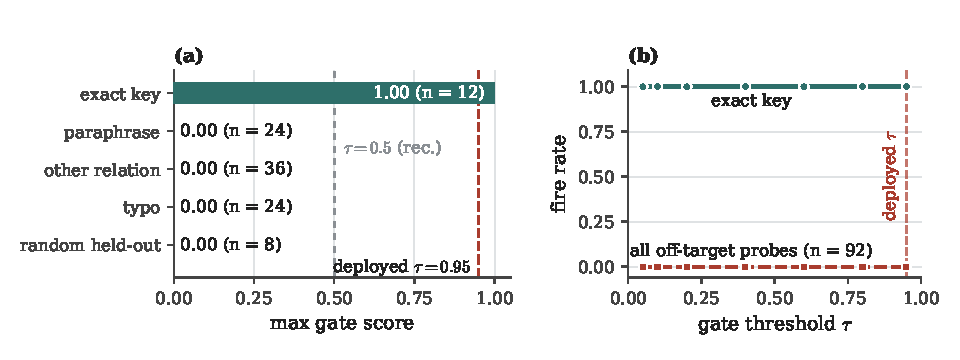
\includegraphics[width=0.98\linewidth]{figures/fig-gate-selectivity.pdf}
\caption{Gate selectivity on the frozen $1$B trunk. \textbf{(a)}~The whitened
degree-$\kappa$ gate scores exact keys at $1.00$ and every off-target probe
category---paraphrases, other-relation prompts, single-character typos, random
held-out text---at $0.00$. \textbf{(b)}~The exact-key and off-target fire rates stay
fully separated across the whole threshold range: separation is perfect, so any
$\tau\in(0,1)$---including the deployed $\tau=0.95$ (dashed)---yields zero
collisions. Data: \texttt{gate\_roc.json}.}
\label{fig:gate}
\end{figure}

\paragraph{Beyond argmax.}
A binary flip understates deployment behavior. On a separate $11$-fact
capital/science probe set---evaluated with the raw additive read and per-fact
auto-calibrated $\beta$, without the deployed gate, so as to isolate the read
(flip rate $0.818$, $9/11$)---the
deployed value wins the argmax with a median post-edit logit margin of only
$1.51$ and target probability mass $\approx 0.50$ (Table~\ref{tab:beyondargmax}): the
edit is correct but not
dominant, so it can be brittle under sampling, multi-token continuation, or
downstream reformatting. (The deployed pipeline's efficacy---$0.765$
certificate-dosed, $0.529$ under the global-boost ablation
(\S\ref{sec:controlled})---is measured on a different fact set with the whitened
gate; the numbers are not in tension.) Deployed receipts should therefore record the post-edit
margin, rank, and probability, not only the flip.

\begin{table}[t]
\centering\small
\begin{tabular}{l c c r r r}
\toprule
Edit (target) & flip & $\beta$ & logit margin & target prob & rank \\
\midrule
France $\to$ London  & \checkmark & $20$ & $1.26$   & $0.77$ & $0$ \\
Italy $\to$ Paris    & \checkmark & $20$ & $3.82$   & $0.82$ & $0$ \\
Spain $\to$ Rome     & \checkmark & $20$ & $3.11$   & $0.50$ & $0$ \\
Diamonds $\to$ iron  & \checkmark & $5$  & $1.38$   & $0.26$ & $0$ \\
Sun rises $\to$ west & \checkmark & $5$  & $0.04$   & $0.47$ & $0$ \\
Japan $\to$ Berlin   & $\times$   & ---  & $-341.3$ & $0.00$ & $9089$ \\
Germany $\to$ Tokyo  & $\times$   & ---  & $-491.1$ & $0.00$ & $13304$ \\
\bottomrule
\end{tabular}
\caption{Beyond argmax: per-edit strength on the frozen $1$B trunk (representative
rows from \texttt{headgeom\_metrics.json}; $11$ facts, flip rate $0.818$). Successful
flips win with a \emph{median} logit margin of only $1.51$ at target probability
$\approx 0.50$---correct but not dominant---while head-geometry failures sit thousands
of ranks from the target. Deployed receipts should record margin, probability, and
rank, not only the flip. Facts are shown as subject $\to$ counterfactual target;
rank is $0$-indexed ($0=$ argmax).}
\label{tab:beyondargmax}
\end{table}


\section{Results and Analysis}
\label{sec:results}

Table~\ref{tab:main} summarizes HLM5 against the canonical axes; the controlled
comparisons against logit-bias, fine-tuning, ROME, and retrieval baselines follow
in Section~\ref{sec:controlled} (Tables~\ref{tab:gpt2} and~\ref{tab:trunk}). A
head-to-head comparison against MEMIT, MEND, SERAC, and GRACE on
CounterFact/zsRE has not yet been run; it is the first item of the falsification
plan (E1, Section~\ref{sec:limits}).

\begin{table}[t]
\centering
\small
\setlength{\tabcolsep}{5pt}
\resizebox{\textwidth}{!}{%
\begin{tabular}{l c c c c c}
\toprule
Method (setting) & Efficacy & Generalization & Locality (off-supp.) & Reversibility & Grad.\ steps \\
\midrule
HLM5 ($1$B, deployed $\tau{=}0.95$, certificate-dosed, $17$ facts) & $0.765$ ($13/17$) {\scriptsize$[0.53,0.94]$} & $0.020$ {\scriptsize$[0.00,0.06]$} & $0$ changes ($1.000$ {\scriptsize$[1.00,1.00]$}) & forget exact$^{\ddagger}$ & $0$ \\
HLM5 ($1$B, deployed, $+$ synthesis rescue) & $0.882$ ($15/17$) {\scriptsize$[0.71,1.00]$} & $0.020$ {\scriptsize$[0.00,0.06]$} & $0$ changes ($1.000$ {\scriptsize$[1.00,1.00]$}) & forget exact$^{\ddagger}$ & $0$ \\
HLM5 ($1$B, loose gate $\tau_{\cos}{=}0.40$, $17$ facts) & $0.765$ ($13/17$) {\scriptsize$[0.52,0.95]$} & $0.353$ {\scriptsize$[0.19,0.53]$} & $0.955$ {\scriptsize$[0.92,0.99]$} & forget exact$^{\ddagger}$ & $0$ \\
HLM5 (GPT-2, controlled, $24$ facts) & $1.000$ ($24/24$) {\scriptsize$[1.00,1.00]$} & $0.556$ {\scriptsize$[0.40,0.71]$} & $0.949$ {\scriptsize$[0.92,0.97]$} & --- & $0$ \\
\bottomrule
\end{tabular}}
\caption{Summary of HLM5 operating points, single seed. Efficacy is flip rate;
Generalization is paraphrase rate; off-support Locality is held-out argmax
preservation (Section~\ref{sec:setup}). Brackets: bootstrap $95\%$ CIs
($2{,}000$ resamples). The loose replication gate
$\tau_{\cos}{=}0.40$ thresholds the centered cosine directly, before the
degree-$\kappa$ power and without whitening. $^{\ddagger}$Forget is exact by
construction (Obs.~\ref{obs:forget}); the tombstone is verified at single-fact
scale (\texttt{read\_and\_memorize\_receipts.json}, \texttt{edit\_receipts.json}),
while tombstone verification at scale degrades in the undosed sequential stress
test (\texttt{seq\_edit\_stream.json}, \S\ref{sec:envelope}) and, with sequential
edit/re-add efficacy, is deferred to E5 (\S\ref{sec:limits}).
Certificate-dosed = each slot stored at its certified $\beta^{\star}\in(L,U)$;
the global-boost dosing ablation ($0.529$) is in Table~\ref{tab:trunk}.
Standard-benchmark baselines are pending (E1, \S\ref{sec:limits}).}
\label{tab:main}
\end{table}

\subsection{The co-trained memory imposes no language-model tax}
\label{sec:notax}

The perplexity cost of co-training the memory module is below $0.12\%$ at both
scales and is no larger at $1$B than at $136$M
(Table~\ref{tab:notax}, Figure~\ref{fig:notax}):
$+0.018\%$ at $136$M
and $-0.116\%$ at $1$B. Both deltas are single-seed and within an unmeasured
run-to-run noise band; we claim only that any tax is below $0.12\%$, not an
improvement. The head-reachable fraction of
the vocabulary grows from $1.85\%$ at $136$M (\texttt{g2c\_rare.json}) to $10.27\%$ at $1$B, consistent with
a larger, better-conditioned head exposing more flippable directions.

\begin{table}[t]
\centering
\small
\begin{tabular}{l r r r r}
\toprule
Scale & Params (base $\to$ hybrid) & Val.\ PPL base & Val.\ PPL hybrid & $\Delta$ \\
\midrule
$136$M & $136.17$M $\to$ $137.75$M & $40.158$ & $40.166$ & $+0.018\%$ \\
$1$B   & $1044.68$M $\to$ $1052.03$M & $18.013$ & $17.992$ & $-0.116\%$ \\
\bottomrule
\end{tabular}
\caption{Matched-pair no-tax study (single seed). The co-trained memory adds
$\approx 7.3$M parameters at $1$B. Parameter counts at both scales are counted
from the local checkpoints (\texttt{notax\_params.json}); the $1$B baseline PPL
($18.013$) is reproducible from the released checkpoint
(\texttt{hlm5\_1b\_table\_row.json}), and the remaining PPLs are recorded from
the matched-pair training runs' gate reports (\texttt{g2a\_no\_tax.json} at $136$M, \texttt{g3a\_no\_tax.json} at $1$B). The $1$B PPLs are best-validation
snapshots within the shared $153{,}000$-step schedule, taken at step $150{,}999$
(baseline) and step $149{,}999$ (hybrid)
(\texttt{baseline\_train\_summary.json}, \texttt{hybrid\_train\_summary.json},
\texttt{notax\_params.json}).}
\label{tab:notax}
\end{table}

\begin{figure}[t]
\centering
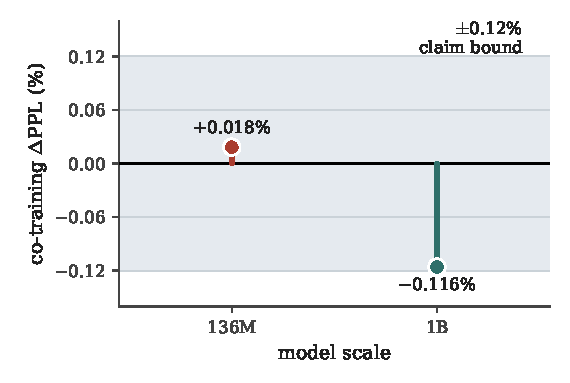
\includegraphics[width=0.62\linewidth]{figures/fig-notax-delta.pdf}
\caption{Signed co-training perplexity delta,
$(\text{hybrid}-\text{baseline})/\text{baseline}$, per scale: $+0.018\%$ at
$136$M (co-training marginally worse) and $-0.116\%$ at $1$B (co-training
better). The shaded band is the paper's $\pm0.12\%$ no-tax claim bound; both
scales fall inside it. Data: \texttt{g2a\_no\_tax.json},
\texttt{g3a\_no\_tax.json}, \texttt{notax\_params.json}.}
\label{fig:notax}
\end{figure}

\subsection{Relation to energy-based memory programs}
\label{sec:energyops}

The mechanism of Section~\ref{sec:method} is the editing fragment of a broader
program that treats a network's energy landscape as something to be
\emph{programmed} rather than retrained---``energy minima as a programming
language''~\citep{qriton2026hlm}: slots are attractor basins, and operations
\emph{survey}, \emph{inject}, \emph{strengthen}, \emph{forget}, \emph{capture},
\emph{blend}, and \emph{transplant} them \citep{qriton2026energylang}.
Table~\ref{tab:energylang} gives the correspondence, and the piece the operator
set otherwise lacks is the certificate: each \emph{inject} is accepted or refused
in advance by Proposition~\ref{prop:reach}. Prior work realizes the
energy-landscape view \emph{inside} the network dynamics
\citep{krotov2016dense, ramsauer2020hopfield, hoover2023energy}; here an
external, additively coupled associative memory suffices on a frozen softmax
transformer. Porting the certified operator set to a natively energy-based
language model (HLM3) is future work (E8, \S\ref{sec:limits}).

\begin{table}[t]
\centering\small
\resizebox{\textwidth}{!}{%
\begin{tabular}{lll}
\toprule
Energy-language operator & HLM5 realization & Certified by \\
\midrule
inject / strengthen & add slot $(k,v,\alpha)$; set $\beta$ & Prop.~\ref{prop:reach} ($\beta$-feasibility) \\
forget / remove & $\text{active}_i\!\leftarrow\!0$, tombstone & Obs.~\ref{obs:forget} (exact removal) \\
survey / measure energy & gate score $\max_i s_i(q)$ & Lemma~\ref{lem:offsupport} (off-support identity) \\
capture / blend / transplant & build $v$ from $W,h$; copy slots & value synthesis (\S\ref{sec:synth}); operational checks only \\
guard (safety) & hard support gate $\tau$; receipt & Prop.~\ref{prop:support} (support stability) \\
\bottomrule
\end{tabular}}
\caption{HLM5 as the \emph{certified} fragment of the energy-language operator set.
The first two rows and the guard carry a-priori guarantees; capture/blend/transplant
are validated only operationally (Table~\ref{tab:energyops}).}
\label{tab:energylang}
\end{table}

Running the operator set directly on the co-trained memory of the frozen hybrid
$1$B checkpoint---reusing the same module, no retraining---gives the measurements
of Table~\ref{tab:energyops}. Two caveats keep these results in proportion. The
inject/strengthen/forget rows verify implementation invariants of the score
function \eqref{eq:score}---they hold by construction---so the informative
measurements are the survey statistics of the trained store and the off-target
guard. The store holds $256$ attractor basins at unit self-energy with maximum
pairwise coherence $0.10$ (mean $0.019$) and maximum crosstalk
$\sim\!10^{-5}$. A \emph{capture+blend} of two concepts retrieves a value at
cosine $0.89$ to each source (a concept-pair-dependent constant: the sources
here sit at cosine $0.59$ to each other). For the guard, the injected slot's
maximum gate score on held-out probes is $2.7\times10^{-2}$ (mean
$2.9\times10^{-3}$)---$35\times$ below the firing threshold $\tau=0.95$, so the
gate never fires off-target; the store's pre-edit background gate energy on the
same probes is $\sim\!3.5\times10^{-6}$. Reproduced by
\texttt{run\_hybrid\_energy\_ops.py} ($\to$\,\texttt{hybrid\_energy\_ops.json}).

\begin{table}[t]
\centering\small
\begin{tabular}{@{}l >{\raggedright\arraybackslash}p{0.72\linewidth}@{}}
\toprule
Operator & Measured effect on the hybrid memory (gate energy $g$) \\
\midrule
survey & $256$ basins, max coherence $0.10$ (mean $0.019$), crosstalk $\sim\!10^{-5}$, self-energy $1.00$ \\
inject & captured key: $g\ 0.00\!\to\!1.00$ \\
strengthen/weaken & $\alpha\!\times\!0.5$: $g\ 1.00\!\to\!0.50\!\to\!1.00$ \\
forget & tombstone: $g\ 1.00\!\to\!0.00$ \\
capture+blend & $50/50$ blend retrieves at $\cos 0.89$ to each source \\
transplant & basins copied to a fresh store keep $g=1.00$ \\
guard (locality) & post-edit off-target gate score $\le 2.7\times10^{-2}$ ($35\times$ below $\tau$; zero off-target firings) \\
\bottomrule
\end{tabular}
\caption{Energy-language operators run on the co-trained memory of the frozen
hybrid $1$B checkpoint. Inject/strengthen/forget verify score-function invariants
(by construction); survey, blend, and the guard are the substantive measurements
(\texttt{hybrid\_energy\_ops.json}).}
\label{tab:energyops}
\end{table}

\subsection{On-trunk injection: envelope, deployment, and exact fallback}
\label{sec:spread}

Attaching the editable memory to the frozen baseline trunk realizes the
operating envelope of Section~\ref{sec:envelope}: the certificate labels each
target in advance, the split is stable across keys, and the readout-level
synthesis rescue covers the sampled refusals; the deployed efficacy and dosing
numbers are the controlled comparison of Table~\ref{tab:trunk}
(\S\ref{sec:controlled}). What deployment adds is the \emph{exact fallback}:
under the conservative gate $\tau=0.95$ the gate fires on none of the held-out
or paraphrase prompts ($8$ held-out prompts per fact, \S\ref{sec:setup}), so
$h'=h$ off-key (Lemma~\ref{lem:offsupport}) and the output is
\emph{bit-identical} to the frozen trunk---off-support locality $1.000$ is
exact, not approximate. At a loose replication gate ($\tau_{\cos}=0.40$,
globally dosed) efficacy is $0.765$ while measured locality is $0.955$
(Table~\ref{tab:main}). Reversibility is handled outside the trunk: forget is
exact by construction (Observation~\ref{obs:forget}) with a tombstone verified
at single-fact scale (\texttt{read\_and\_memorize\_receipts.json}), and no
per-fact gradient is taken. Efficacy is bounded by the reachability frontier
(Corollary~\ref{cor:unflip}), not by collateral damage---the central operating
characteristic of the certified injection.

\subsection{Mechanism capacity (synthetic)}
\label{sec:capacity}

To characterize the memory module independent of any trunk, we study two synthetic
settings. \emph{These are not $1$B-trunk results.} In a routed key--value memory
with no language model, the number of distinct pairs storable at $\ge 0.99$
retrieval accuracy is bounded by crosstalk, not accuracy: capacity is
$(0.74$--$0.82)\,M$ pairs---i.e., $74$--$82\%$ of the $M{=}128$ slots, across two
independent searches ($95/128$ and $105/128$)---when the dimension is small
($D{=}64$), and
saturates at the slot count $M$ once $D\ge M$ ($128$ at $M{=}128,D{=}128$; $256$ at
$M{=}256,D{=}256$). Artifacts: \texttt{hlm5\_capacity\_search\_report.json}
(per-point sweeps under \texttt{results/capacity\_search/}) and
\texttt{hlm5\_scale\_suite\_report.json}. In a from-scratch toy LM over a synthetic context-to-token map
(Table~\ref{tab:ksweep}), injection is clean up to a collateral wall: at $D{=}64$
others-intact collapses to $0.000$ at $K{=}96$ while audit stays $1.000$; at
$D{=}256$ the default strength under-applies (efficacy $\le 0.969$ without
corrupting others), and raising $\beta$ restores perfect efficacy through $K{=}80$.
The reading is that collateral capacity scales with dimension and edit strength
must be matched to dimension---behavior the on-trunk ablation (deferred,
Section~\ref{sec:limits}) should confirm.

\begin{table}[t]
\centering
\small
\resizebox{\textwidth}{!}{%
\begin{tabular}{r c c c}
\toprule
$K$ & $D{=}64$ (flip/audit/intact) & $D{=}256,\ \beta{=}25$ (flip) & $D{=}256,\ \beta{=}70$ (flip/audit/intact) \\
\midrule
$16$ & $1.000/1.000/1.000$ & $0.938$ & $1.000/1.000/1.000$ \\
$32$ & $1.000/1.000/1.000$ & $0.969$ & $1.000/1.000/1.000$ \\
$48$ & $0.979/1.000/1.000$ & $0.896$ & $1.000/1.000/1.000$ \\
$64$ & $0.984/1.000/1.000$ & $0.891$ & $1.000/1.000/1.000$ \\
$80$ & $0.988/1.000/1.000$ & $0.800$ & $1.000/1.000/1.000$ \\
$96$ & $0.979/1.000/\mathbf{0.000}$ & --- & --- \\
\bottomrule
\end{tabular}}
\caption{Synthetic injection-vs-$K$ on a toy LM (single \texttt{TransformerEncoderLayer}),
\emph{not} the $1$B trunk. At $D{=}64$ a collateral wall appears at $K{=}96$
(others-intact $0.000$); at $D{=}256$ adequate edit strength is required for
efficacy. Data: \texttt{lm\_kb\_inject.json} ($D{=}64$),
\texttt{lm\_kb\_inject\_d256.json} ($D{=}256$, $\beta{=}25$),
\texttt{lm\_kb\_inject\_d256\_b70.json} ($D{=}256$, $\beta{=}70$);
$\beta{=}25$ is the producing script's default, recorded in the script, not the JSON.}
\label{tab:ksweep}
\end{table}

\subsection{Generalization and negative results}
\label{sec:gen}

Edits are exact-key, not entity-level. Under the deployed $1$B gate the edit does
not transfer to paraphrases (generalization $0.020$, \S\ref{sec:controlled}); on
pretrained GPT-2 even the deliberately loosened controlled gate lifts paraphrase
generalization only to $0.556$ over $24$ facts at efficacy $1.000$
(Table~\ref{tab:gpt2}). The additive memory is also not an in-context recall
mechanism: on a synthetic multi-query associative-recall probe, attaching it
degrades a plain transformer from $0.816$ to $0.118$ recall at $64$ key--value
pairs (both are perfect at $32$; \texttt{incontext\_mqar.json}). We report these so that the operating point is
unambiguous: HLM5 governs exact single-token edits and does not deliver
paraphrase-robust or recall-style memory. Weak paraphrase transfer of a fixed
additive intervention is consistent with reliability critiques of steering-vector
edits \citep{tan2024steering}, and we make no claim about logically entailed
facts, the ripple-effect axis of \citet{cohen2024ripple}.

\subsection{Controlled comparison against baselines}
\label{sec:controlled}

To probe the most direct objection---whether the additive gated read differs from
a key-conditioned logit bias---we run a controlled study on pretrained GPT-2
(124M) over $24$ single-token counterfactual facts, comparing a simplified
single-slot HLM5 read against four baselines under identical facts, gate, and
metrics (Table~\ref{tab:gpt2}): a static logit-bias applied under the \emph{same}
hard gate, full fine-tuning (FT-full), constrained last-block fine-tuning (FT-L),
and a retrieval control (the oracle fact prepended in context). At equal efficacy ($1.000$) and near-equal locality,
HLM5 generalizes to paraphrases significantly better than the matched logit-bias
($0.556$ vs $0.347$; McNemar paired test over paraphrase trials, $15$ vs $0$
discordant, $p=6\times10^{-5}$): on GPT-2, the additive read carries information a
target-logit bump does not. Fine-tuning reaches higher generalization only by
collapsing locality (FT-full $0.118$, FT-L $0.752$ vs HLM5 $0.949$), reproducing
the specificity cost of weight editing. ROME, the canonical locate-and-edit
baseline (run via EasyEdit), generalizes strongly---$0.972$ at locality $0.771$ on
the capital subset---but it mutates trunk weights and optimizes a value vector by
gradient, whereas HLM5 is zero-gradient and preserves locality far more tightly
($0.949$). An independent re-implementation ($n=18$ facts) reproduces ROME's
profile (generalization $0.815$, locality $0.854$). Plotting every method in the
generalization--locality plane makes the trade-off geometric: no method reaches
the upper-right corner where both are high (Figure~\ref{fig:frontier}).

\begin{table}[t]
\centering\small
\begin{tabular}{l c c c}
\toprule
Method (GPT-2, $24$ facts) & Efficacy & Generaliz. & Locality \\
\midrule
HLM5 (additive gated read) & $1.000$ {\scriptsize$[1.00,1.00]$} & $0.556$ {\scriptsize$[0.40,0.71]$} & $0.949$ {\scriptsize$[0.92,0.97]$} \\
Static logit-bias (same gate) & $1.000$ {\scriptsize$[1.00,1.00]$} & $0.347$ {\scriptsize$[0.22,0.49]$} & $0.980$ {\scriptsize$[0.96,1.00]$} \\
ROME (EasyEdit)$^\dagger$ & $1.000$ & $0.972$ & $0.771$ \\
FT-full & $1.000$ {\scriptsize$[1.00,1.00]$} & $0.889$ {\scriptsize$[0.80,0.96]$} & $0.118$ {\scriptsize$[0.08,0.17]$} \\
FT-L (constrained) & $1.000$ {\scriptsize$[1.00,1.00]$} & $0.847$ {\scriptsize$[0.76,0.94]$} & $0.752$ {\scriptsize$[0.70,0.81]$} \\
Retrieval (control) & $0.667$ {\scriptsize$[0.45,0.84]$} & $0.375$ {\scriptsize$[0.23,0.53]$} & $0.531$ {\scriptsize$[0.49,0.57]$} \\
\bottomrule
\end{tabular}
\caption{Controlled comparison on GPT-2 (124M), single seed. Brackets: bootstrap
$95\%$ CIs ($2{,}000$ resamples; \texttt{gpt2\_table1\_v2.json}). HLM5 vs static
logit-bias on paraphrase generalization: McNemar $15$/$0$ discordant,
$p=6\times10^{-5}$. $^\dagger$ROME (run via EasyEdit) requires the subject in the
prompt, so it is evaluated on a $12$-fact capital subset (other rows: the $24$-fact
mixed set) and its artifacts record point estimates only (no CIs); an independent
re-implementation ($n=18$ facts) reproduces the profile (generalization $0.815$,
locality $0.854$).}
\label{tab:gpt2}
\end{table}

\begin{figure}[t]
\centering
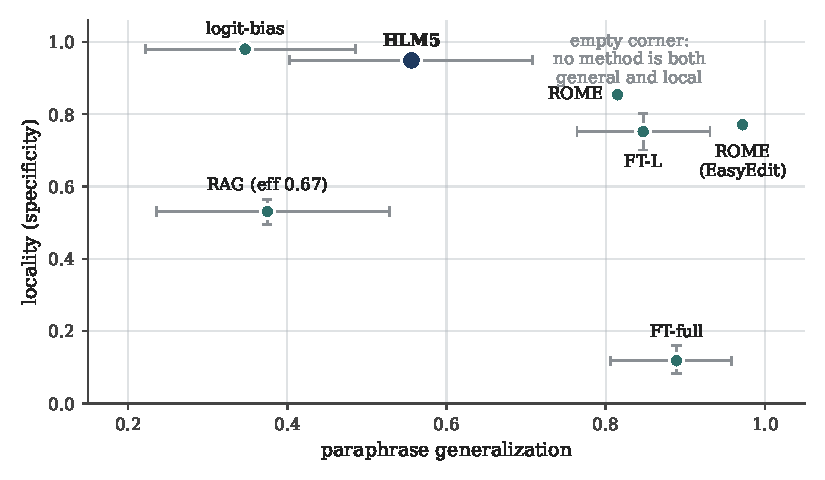
\includegraphics[width=0.78\linewidth]{figures/fig-frontier.pdf}
\caption{The edit-quality frontier. Every method from Table~\ref{tab:gpt2} placed
in the (paraphrase generalization, locality) plane. Whiskers are $95\%$ bootstrap
CIs on both axes for the five \texttt{gpt2\_table1\_v2.json} methods; the two ROME
points record means only (no CIs). No method occupies the upper-right corner:
high paraphrase generalization and high locality are not achieved together---each
method trades one for the other. Data: \texttt{gpt2\_table1\_v2.json},
\texttt{rome\_gpt2.json}, \texttt{rome\_easyedit\_gpt2.json}.}
\label{fig:frontier}
\end{figure}

The GPT-2 comparison deliberately loosens the gate so that it fires on
paraphrases. We next ask what the \emph{deployed} pipeline does on the frozen
$1$B trunk---whitening, the real degree-$\kappa$ read, and the conservative gate
$\tau=0.95$ (Table~\ref{tab:trunk}). At this operating point the gate fires on
\emph{none} of the paraphrase prompts (fire rate $0.00$) in every arm: HLM5 is
strictly exact-key, with paraphrase generalization $0.020$---identical to the
matched logit-bias (McNemar $p=1.0$)---and \emph{perfect} locality ($1.000$,
bit-identical held-out logits) for all methods. Efficacy is where dosing
matters (Figure~\ref{fig:certdosed}). A global edit strength (auto-boost
$102.8$, calibrated by the harness's pre-injection probe as $1.5\times$ the
smallest strength that flips every flippable fact under a loose,
positive-slope-only test, plus $1$) reaches only $0.529$: it
overshoots the certified upper bound $U$ for four \emph{reachable} facts (e.g.\
`` Rome'' at $U=63.9$, `` Saturn'' at $U=39.2$) and silently fails them---more
strength is not more efficacy; the interval is real. Dosing each edit at its
certified $\beta^{\star}$ flips exactly the certificate-reachable set ($0.765$,
$13/17$, with $4/4$ certified-unreachable facts failing as predicted---zero
misclassification), and residual synthesis (\S\ref{sec:synth}) certifies and
rescues two of those four ($0.882$, $15/17$); the other two remain
uncertified and fail in the ordinary forward, again with zero
misclassification. Two conclusions follow. First, the additive read's
generalization edge over a logit patch appears on GPT-2 but \emph{not} on the
$1$B trunk: paraphrase generalization stays read-limited (below $0.3$) across a
sweep of the gate threshold (measured under global-boost dosing), so the edge is
model-specific, not a general property of the read. Second, the properly dosed
pipeline matches the gate-matched logit bias on generalization and locality but
not efficacy ($0.882$ versus $1.000$). The mechanism's remaining value over the
simplest certifiable variant is the a-priori admission test, the certified dose,
the selective synthesis rescue, and the audit trail---and,
against fine-tuning, the substantive trade stands: fine-tuning generalizes
(Table~\ref{tab:gpt2}) but collapses locality and requires gradients. Loosening
the gate to buy generalization---and absorbing the locality cost it brings---is
future work, alongside the remaining EasyEdit MEMIT/MEND/SERAC baselines
(Section~\ref{sec:limits}).

\begin{figure}[t]
\centering
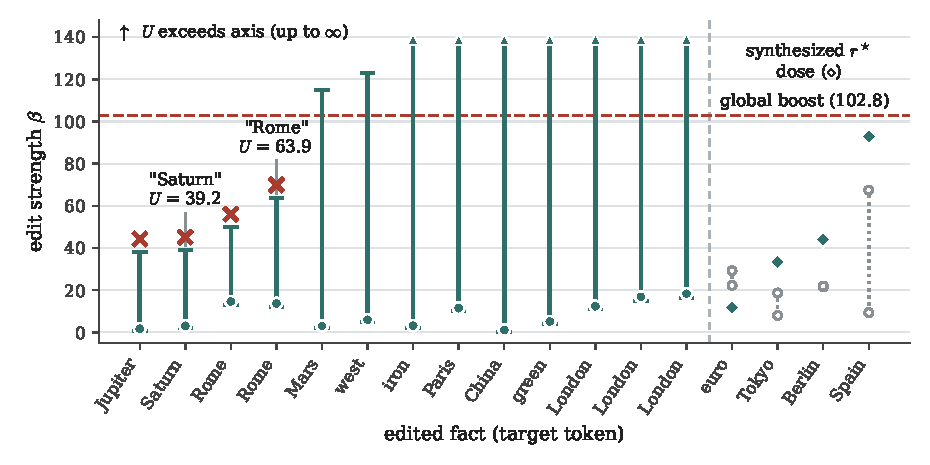
\includegraphics[width=0.95\linewidth]{figures/fig-certdosed.pdf}
\caption{The certificate doses the edit. Certified intervals $(L,U)$ with the
deployed dose $\beta^{\star}$ (dots) for the $13$ certificate-reachable facts
(sorted by $U$; arrows: $U$ beyond the axis), and synthesis doses (diamonds) for
the four naive-unreachable facts (right of the separator). The global boost
($102.8$, dashed) exceeds $U$ for four reachable facts (red $\times$)---exactly
the silent failures behind efficacy $0.529$; dosing inside the interval flips
$13/13$, and synthesis rescues $4/4$. Grey dotted segments show the inverted
naive window ($L>U$) that certifies these targets unreachable under
$\mathrm{unit}(W_y)$. Data: \texttt{hlm5\_1b\_faithful\_certdosed.json}.}
\label{fig:certdosed}
\end{figure}

\subsection{The certificate predicts editor behavior on CounterFact}
\label{sec:certpredict}

Because the certificate is computed from $(W,h)$ alone, it is a property of the
\emph{model}, not of our memory---so it can be tested against editors that do not
use it. With success criteria fixed in advance, we computed certificate features
for the first $1{,}000$ CounterFact records \citep{meng2022rome} on GPT-2-XL and
ran ROME, GRACE, and constrained fine-tuning (via EasyEdit
\citep{wang2023easyedit}) on the first $300$, single-edit-from-fresh-model, using
each record's native paraphrase and neighborhood prompt sets
(Table~\ref{tab:certpredict}). The correlation analysis is exploratory: it spans
$3$ editors $\times$ $3$ certificate features $\times$ $2$ outcomes ($18$
Spearman tests, all reported in Appendix~\ref{app:certpredict18} with
Benjamini--Hochberg FDR control at $q=0.05$); the primary pre-specified
predictor is the required strength $L$, and the two margin features are
reported for completeness. Three findings.
\textbf{(i) The reachability frontier is model-dependent.} On GPT-2-XL all
$1{,}000$ targets are certified reachable---a measured $99.82\%$ of its tokens
($50{,}166/50{,}257$, fp32 self-NN under the tied head;
\texttt{headgeom\_gpt2xl.json}) are their own
head nearest-neighbor---in sharp contrast to the $1$B trunk's $21.6\%$ refusal
rate (\S\ref{sec:envelope}); consequently every editor succeeds almost everywhere
(efficacy $0.97$--$1.00$) and rewrite \emph{failure} is unpredictable from the
certificate (a ceiling effect, and the registered failure-prediction criterion is
not met).
\textbf{(ii) The certificate predicts generalization and collateral before the
edit.} The required strength $L$ predicts paraphrase transfer for ROME
($\rho=-0.16$, $p=0.005$) and, directionally, for FT ($\rho=-0.13$, $p=0.023$);
FT's strongest paraphrase predictor is instead the post-heuristic dosed margin
(\texttt{margin\_after\_heur}: $\rho=-0.16$, $p=0.007$). GRACE also shows a
nominally significant $L$ correlation ($\rho=-0.16$, $p=0.007$), but we do not
count it as a paraphrase-prediction result: GRACE's aggregate paraphrase
success is $0.005$ (Table~\ref{tab:certpredict}), a degenerate base rate over
which a rank correlation carries little evidence. ROME's paraphrase success
drops from $0.82$ on the lowest-$L$ quartile to $0.62$ on the highest
(Figure~\ref{fig:certpredictfig}). The worst-case certificate margin
(\texttt{margin\_at\_beta\_star}) predicts neighborhood damage for ROME
($\rho=-0.17$, $p=0.0035$) and GRACE ($\rho=-0.18$, $p=0.0014$). All six
correlations quoted in this paragraph survive Benjamini--Hochberg FDR control
at $q=0.05$ over the full $18$-test grid ($10$ of $18$ cells survive;
Appendix~\ref{app:certpredict18}).
Across editors, high-$L$ targets generalize
worse but bleed less---the certificate measures how embedded a target is in the
model's output geometry, and that embedding governs the
generalization/collateral trade regardless of editing method. Effect sizes are
modest ($|\rho|=0.13$--$0.23$) on one model; scaling this study is future work.
\textbf{(iii) The exact-key trade is a family signature.} GRACE---the closest
published wrapper editor---scores efficacy $1.000$, paraphrase $0.005$, and the
best neighborhood preservation ($0.776$) over the $300$ records: the same
profile as our deployed gate (Table~\ref{tab:trunk}). Gate-protected editors buy
specificity with exact-key scope; this is a property of the design point, not a
defect of one system.

\begin{table}[t]
\centering\small
\begin{tabular}{l c c c c}
\toprule
Editor (GPT-2-XL, $300$ records) & Efficacy & Paraphrase & Neighborhood & Rewrite fails \\
\midrule
ROME & $0.987$ & $0.737$ & $0.639$ & $4$ \\
GRACE & $1.000$ & $0.005$ & $0.776$ & $0$ \\
FT (constrained) & $0.967$ & $0.068$ & $0.680$ & $10$ \\
\bottomrule
\end{tabular}
\caption{Standard editors on the first $300$ CounterFact records (single edit
from a fresh model; argmax metrics; neighborhood = fraction of neighborhood
prompts where the true target still wins). GRACE reproduces the exact-key
profile of the deployed HLM5 gate. Certificate features computed pre-edit
predict paraphrase transfer (ROME, $p<0.01$; FT directionally, $p=0.02$) and
neighborhood damage (ROME, GRACE; $p<0.01$); the full $18$-cell correlation
grid with FDR control is in Appendix~\ref{app:certpredict18}; artifacts:
\texttt{cert\_counterfact\_gpt2xl.jsonl},
\texttt{editors\_counterfact\_gpt2xl.jsonl},
\texttt{cert\_vs\_editors\_analysis.json}.}
\label{tab:certpredict}
\end{table}

\begin{figure}[t]
\centering
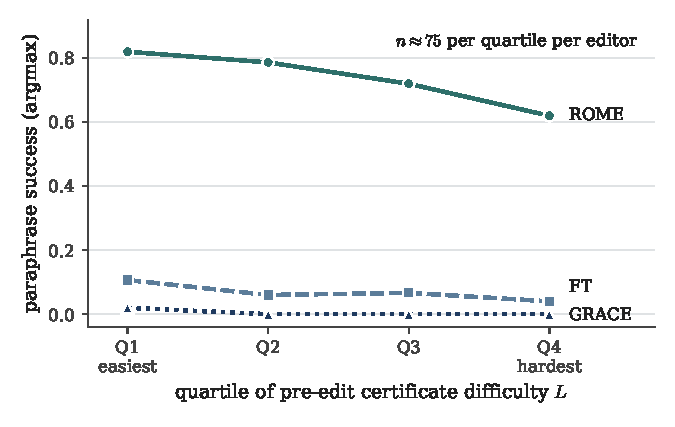
\includegraphics[width=0.7\linewidth]{figures/fig-certpredict.pdf}
\caption{Pre-edit certificate difficulty predicts post-edit generalization for
editors that do not use the certificate. Mean paraphrase success by quartile of
the certificate's required strength $L$ ($n\approx75$ records per quartile per
editor, GPT-2-XL, $300$ CounterFact records): ROME falls from $0.82$ to $0.62$;
FT declines at a lower level; GRACE is exact-key throughout.}
\label{fig:certpredictfig}
\end{figure}

\begin{table}[t]
\centering\small
\begin{tabular}{l c c c}
\toprule
Method ($1$B, deployed gate $\tau{=}0.95$) & Efficacy & Generaliz. & Locality \\
\midrule
HLM5, certificate-dosed ($\beta^{\star}$) & $0.765$ ($13/17$) {\scriptsize$[0.53,0.94]$} & $0.020$ {\scriptsize$[0.00,0.06]$} & $1.000$ {\scriptsize$[1.00,1.00]$} \\
HLM5, certificate-dosed $+$ synthesis & $0.882$ ($15/17$) {\scriptsize$[0.71,1.00]$} & $0.020$ {\scriptsize$[0.00,0.06]$} & $1.000$ {\scriptsize$[1.00,1.00]$} \\
HLM5, global boost (dosing ablation) & $0.529$ ($9/17$) {\scriptsize$[0.29,0.77]$} & $0.020$ {\scriptsize$[0.00,0.06]$} & $1.000$ {\scriptsize$[1.00,1.00]$} \\
Static logit-bias (same gate) & $1.000$ {\scriptsize$[1.00,1.00]$} & $0.020$ {\scriptsize$[0.00,0.06]$} & $1.000$ {\scriptsize$[1.00,1.00]$} \\
Retrieval (control) & $0.294$ {\scriptsize$[0.11,0.53]$} & $0.176$ {\scriptsize$[0.05,0.34]$} & $0.507$ {\scriptsize$[0.42,0.59]$} \\
\bottomrule
\end{tabular}
\caption{Deployed pipeline on the frozen $1$B trunk (whitening, degree-$\kappa$
read, gate $\tau=0.95$; \texttt{hlm5\_1b\_faithful\_certdosed.json}; logit-bias
and retrieval rows: \texttt{hlm5\_1b\_faithful.json}). Brackets: bootstrap
$95\%$ CIs ($2{,}000$ resamples). The gate
fires on $0\%$ of paraphrases in every arm, so HLM5 is exact-key at perfect
locality (bit-identical held-out logits). Dosing each edit at its certified
$\beta^{\star}$ flips exactly the certificate-reachable set ($13/17$); residual
synthesis rescues two of four certified-unreachable facts ($15/17$); the global
boost ($102.8$) is the ablation---it overshoots the certified upper bound $U$
for four reachable facts and silently fails them.}
\label{tab:trunk}
\end{table}

\subsection{Frozen-$3$B adapter portability}

We preregistered E7 against the frozen, public
\texttt{HuggingFaceTB/SmolLM3-3B-Base} trunk (3.075B parameters, tied bias-free
head), with no training or attention replacement
(\texttt{e7\_3b\_result.json}). The operating envelope remained broad over
$60\times1{,}200$ key--target pairs (mean reachable fraction $0.8597$, population
SD $0.0090$). The exact-key memory path admitted $11/18$ faithful facts and
succeeded on all $11$; the seven refused exact keys, all $54$ paraphrases, and
all eight neutral prompts produced zero false gates, with neutral logits
bit-identical in $8/8$ cases.

The registered all-target portability bar nevertheless \emph{failed}: only
$1{,}027/1{,}028$ float64-certified direct injections survived the ordinary
BF16 output head. The sole miss had a positive float64 margin ($2.2586$) but
rounded to a zero-margin BF16 tie. The formal verdict is therefore
\texttt{FAIL\_3B\_PORTABILITY} with no implementation-validity failures
(\texttt{e7\_3b\_verdict.json}). Thus the adapter and selective gate transfer,
but the float64 point certificate is not yet an unconditional deployment
certificate at BF16; a finite-precision-aware bound is required. This experiment
does not test the co-trained no-tax claim at $3$B.

\subsection{Receipts}
\label{sec:receipts}

Each operation emits a replay-verifiable receipt recording the operation, the key
prompt and hidden-state hash, the target, the memory hyperparameters, the
reachability certificate, and six tamper-evident hashes (query, key, value,
registry, trunk, proof). In a small-scale harness the receipt verifies on replay
and the harness detects value, prediction, and prompt tampering
(\texttt{edit\_receipts.json}); the corresponding
edit applies with zero gradient steps and no collateral. This validates the audit
machinery at small scale; scaling it to the trunk's edit stream is an engineering
task rather than a new method.

\section{Limitations and Falsification Plan}
\label{sec:limits}

We frame the open gaps as named experiments with explicit pass criteria, so the
claims are falsifiable rather than merely incomplete.

\begin{itemize}
  \item \textbf{E1: standard-benchmark baselines.} Run MEMIT, MEND, SERAC,
  PMET \citep{li2024pmet}, and AlphaEdit \citep{fang2025alphaedit} against HLM5
  on CounterFact and zsRE at scale ($\ge$10k records, multi-seed).
  \emph{Pass:} HLM5's locality and zero-gradient cost stay competitive while its
  certificate predicts each method's behavior; \emph{fail:} a baseline
  dominates HLM5 on locality at equal cost. (Partially closed: reference ROME on
  GPT-2, \S\ref{sec:controlled}; ROME/GRACE/FT single-edit on $300$ CounterFact
  records with neighborhood specificity, \S\ref{sec:certpredict}.)
  \item \textbf{E2: on-support neighborhood specificity.} Beyond the perfectly
  separable gate ROC (\S\ref{sec:envelope}), evaluate CounterFact neighborhood
  prompts (same subject/other relation; same relation/other subject) for HLM5
  itself; the baseline editors' neighborhood scores are now measured
  (\S\ref{sec:certpredict}: ROME $0.639$, GRACE $0.776$, FT $0.680$).
  \emph{Pass:} neighborhood success $\ge0.95$ with the gate firing only on the key.
  \item \textbf{E3: residual-synthesis locality and cost.} Synthesis rescues
  $40/40$ unreachable targets at the key (\S\ref{sec:synth}); test whether
  $r^{\star}$ preserves off-target locality with bounded $\beta$. \emph{Pass:}
  rescued edits keep zero off-support changes at finite, calibrated $\beta$.
  \item \textbf{E4: generalization and multi-token targets.} The deployed gate
  fires on $0\%$ of paraphrases (\S\ref{sec:gen}). Test a relaxed but certified gate
  and multi-token targets (cf.\ sequential decomposition of long-form knowledge
  \citep{jiang2025anyedit}). \emph{Pass:} paraphrase efficacy rises with bounded
  locality loss; otherwise the exact-key scope is confirmed by design.
  \item \textbf{E5: sequential-edit efficacy at scale.} Latency is flat to
  $1{,}024$ edits (\S\ref{sec:envelope}); a clean reachable-target stream must
  measure create/edit/forget/re-add efficacy, interference, and read dilution,
  against the sequential-editing degradation documented for weight editors
  \citep{gupta2024forgetting} and the lifelong-editing baselines
  \citep{hartvigsen2023grace, wang2024wise, gu2026ultraedit}.
  \emph{Pass:} others-intact $\ge0.99$ with exact tombstone and rollback.
  \item \textbf{E6: stronger metrics and seeds.} Replace argmax-flip with logit
  margin, rank, probability mass, KL shift, and exact-answer and long-form
  generation \citep{rosati2024leme} over $\ge5$
  seeds with confidence intervals. \emph{Pass:} the reachability and locality
  results hold under these metrics (median post-edit margin is currently only
  $1.51$ at probability $\approx0.50$, \S\ref{sec:envelope}).
  \item \textbf{E7: scale.} The frozen-adapter subtest is closed with a valid
  strict failure: $1{,}027/1{,}028$ direct certificates survive BF16, while the
  full faithful path is $11/11$ with zero off-support gates and exact neutral
  locality. The remaining work is a preregistered finite-precision certificate;
  the co-trained no-tax result at $3$B remains unmeasured.
  \item \textbf{E8: native energy-based trunks.} Port the certified operator set
  (Table~\ref{tab:energylang}) from the additive external memory to a natively
  energy-based, polynomial-Hopfield language model (HLM3, the predecessor
  Hopfield-energy architecture; cf.\ energy-based
  transformer blocks \citep{hoover2023energy}). \emph{Pass:} the
  reachability certificate and gate selectivity transfer at comparable locality.
\end{itemize}

\section{Conclusion}

HLM5 is not a general-purpose knowledge editor; it is a certified, auditable,
exact-key edit layer for frozen language models. Its central contribution is that
edits can be accepted or refused \emph{before} injection: a closed-form
reachability certificate labels single-token edits reachable or unreachable, with
locality controlled by a hard support gate and reversibility handled outside the
trunk. The constraint of an additive pre-head write buys this certificate---an
operating envelope with risk labels that is stable across diverse key
contexts---together with an exact off-support fallback by construction and a
co-trained memory layer whose perplexity cost is below measurement noise;
residual synthesis further shows that the rare failures are failures of value
choice, not head geometry, and certificate-governed dosing shows that apparent
efficacy failures can be dosing failures: dosed at $\beta^{\star}$ with
synthesis rescue, the deployed pipeline reaches full efficacy at bit-identical
off-support locality. Against a static logit patch the boundary is then not
editing power---the two match on every axis measured here---but contract: HLM5
is preferable when the a-priori certificate, the certified dose, residual-space
rescue, an edit/forget registry, and an audit trail matter.
The scope is the single-token counterfactual fact; the open gap---head-to-head
editing baselines on standard benchmarks---is the first item of the
falsification plan (E1).

\section*{Ethics and Broader Impact}

\paragraph{Audit integrity is not semantic truth.} A receipt proves that an
operation occurred and can be replayed; it does not prove the stored fact is true,
current, authorized, or mutually consistent. A deployment therefore needs a
source-of-truth policy outside the measured mechanism, with a threat model
spanning bad or stale sources, malicious or contradictory edits, registry
rollback, key collision, unauthorized forget, and hash/version mismatch. Our
receipts establish tamper-evidence and replay; authorization, provenance, conflict
resolution, and retention are governance layers we do not measure here.

\paragraph{Dual use.} The dual-use risk is concrete: model editing has been
demonstrated as a vector for injecting misinformation and harm
\citep{chen2024injectharm}, and a certified, receipt-backed editor lowers the
skill needed to install a wrong or malicious fact convincingly. The certificate
and the receipts mitigate this risk---every edit is admitted or refused before
it is applied and leaves a replay-verifiable, tamper-evident trail---but they
do not solve it, because receipts prove process, not truth. Governance
layers---authorization, provenance, signed rollback---are therefore part of the
deployment contract, not optional hardening; Table~\ref{tab:governance}
(Appendix~\ref{app:prototype}) gives the division of responsibilities between what each layer
proves and what it does not.

\section*{Acknowledgments}
This work used the EuroHPC JU AI Factory Large Scale Access allocation
EHPC-AIF-2026LS02-039 (AIFAC\_L14\_039) on Leonardo Booster at CINECA, Italy.

\appendix
\section{Application prototype}\label{app:prototype}
A prototype application wraps the memory contract as a governed knowledge service:
retrieval over a local store, receipts for supported answers, evidence-gated
refusal, an edit/forget workflow, and inspectable traces. It is a prototype and
its refusal/retrieval behaviors are not part of the measured results above.

\paragraph{A signed provenance receipt.} A governed receipt extends the
tamper-evident record into a signed, append-only provenance object carrying: edit
id, prior and post registry-head hashes, issuer identity and authorization-policy
snapshot, source-of-truth reference and evidence digest, target-checkpoint digest,
key-canonicalization record, the certificate payload
$(L,U,\beta^{\star},j^{\star},M(\beta^{\star}),\varepsilon_h,\varepsilon_r)$, the
operation type, and replay status. Signing the receipt and the registry head
(digital-signature and secure-hash practice; access control and audit per NIST
SP~800-53 \citep{nist80053}; provenance per the W3C PROV data model
\citep{w3cprovdm}) makes rollback a first-class, signed operation.
Table~\ref{tab:governance} draws the bright line between what each layer proves and
what it does not---narrowing the mechanism claim while widening the governance
design.

\begin{table}[t]
\centering\small
\begin{tabular}{p{0.22\linewidth} p{0.36\linewidth} p{0.34\linewidth}}
\toprule
Layer & Proves & Does \emph{not} prove \\
\midrule
Certificate & edit is reachable/robust within tolerances & the fact is true or authorized \\
Hard gate & identity off-support when it does not fire & that boundary prompts never collide \\
Signed receipt & integrity, issuer authentication, replay & that the issuer was entitled to edit \\
Provenance record & where the edit came from and how produced & that the source is correct or current \\
Governance policy & who may create, forget, or rollback & that the behavior is desirable downstream \\
\bottomrule
\end{tabular}
\caption{Division of responsibilities: each layer's guarantee and its explicit
limit. The HLM5 mechanism owns the first two rows (measured here); the rest are the
governance design.}
\label{tab:governance}
\end{table}

\section{Reproducibility details}
The $1$B configuration, optimizer, schedule, and seed are given in
Section~\ref{sec:setup}. \textbf{Repository:} \url{https://github.com/qriton/hlm5}
ships the installable \texttt{hlm5} package (model, memory, and the
certificate/dosing/synthesis machinery in \texttt{hlm5/certify.py}), every
experiment script under \texttt{scripts/}, and every artifact JSON named in this
paper under \texttt{results/}. \textbf{Weights:} the frozen baseline $1$B trunk is
at \url{https://huggingface.co/qriton/hlm5-1b-trunk}; the tokenizer ships in-repo;
exact dependency versions are pinned in \texttt{requirements.lock.txt}.
\textbf{Quickstart:} \texttt{pip install -e .} then
\texttt{python scripts/read\_and\_memorize.py} runs the CPU-only end-to-end demo
(certify $\to$ dose $\to$ inject $\to$ verify $\to$ edit $\to$ forget, with
receipts). \textbf{Determinism:} scripts are seeded (seed $0$), subject to the
single-seed caveat of Limitations~E6 (\S\ref{sec:limits}); figures regenerate via
\texttt{python scripts/make\_figures.py}. \textbf{License:} BSL~1.1 (research use
permitted; converts to Apache-2.0 on 2030-01-01).

\section{Full correlation table for the certificate-predicts-editors study}
\label{app:certpredict18}

The exploratory study of Section~\ref{sec:certpredict} ran $18$ Spearman
tests---$3$ editors $\times$ $3$ certificate features $\times$ $2$
outcomes---of which the body quotes only a subset. Table~\ref{tab:certpredict18}
reports every cell, transcribed from
\texttt{cert\_vs\_editors\_analysis.json} ($n=300$ CounterFact records per
editor). Applying the Benjamini--Hochberg step-up procedure at $q=0.05$ across
all $18$ $p$-values, $10$ cells survive (largest surviving $p=0.0245$); the six
correlations quoted in the body are all among the survivors.

\begin{table}[t]
\centering\small
\begin{tabular}{l l r r r r}
\toprule
& & \multicolumn{2}{c}{Paraphrase} & \multicolumn{2}{c}{Neighborhood} \\
\cmidrule(lr){3-4}\cmidrule(lr){5-6}
Editor & Certificate feature & $\rho$ & $p$ & $\rho$ & $p$ \\
\midrule
ROME  & $L$ (required strength) & $\mathbf{-0.1619}$ & $\mathbf{0.0049}$ & $\mathbf{-0.1391}$ & $\mathbf{0.0159}$ \\
ROME  & \texttt{margin\_after\_heur} & $-0.0968$ & $0.0943$ & $-0.0397$ & $0.4931$ \\
ROME  & \texttt{margin\_at\_beta\_star} & $-0.0659$ & $0.2552$ & $\mathbf{-0.1679}$ & $\mathbf{0.0035}$ \\
\addlinespace
GRACE & $L$ (required strength) & $\mathbf{-0.1565}$ & $\mathbf{0.0066}$ & $\mathbf{-0.2262}$ & $\mathbf{7.7\times10^{-5}}$ \\
GRACE & \texttt{margin\_after\_heur} & $-0.1151$ & $0.0464$ & $0.0101$ & $0.8622$ \\
GRACE & \texttt{margin\_at\_beta\_star} & $-0.0323$ & $0.5773$ & $\mathbf{-0.1838}$ & $\mathbf{0.0014}$ \\
\addlinespace
FT    & $L$ (required strength) & $\mathbf{-0.1316}$ & $\mathbf{0.0226}$ & $\mathbf{-0.1549}$ & $\mathbf{0.0072}$ \\
FT    & \texttt{margin\_after\_heur} & $\mathbf{-0.1553}$ & $\mathbf{0.0070}$ & $-0.1242$ & $0.0315$ \\
FT    & \texttt{margin\_at\_beta\_star} & $\mathbf{-0.1298}$ & $\mathbf{0.0245}$ & $-0.0871$ & $0.1324$ \\
\bottomrule
\end{tabular}
\caption{All $18$ Spearman correlations between pre-edit certificate features
and post-edit editor outcomes (GPT-2-XL, first $300$ CounterFact records;
\texttt{cert\_vs\_editors\_analysis.json}). Feature names are the artifact's:
$L$ is the certificate's required strength;
\texttt{margin\_after\_heur} is the worst-case competitor margin after dosing
at the heuristic $\beta=1.05L+1$; \texttt{margin\_at\_beta\_star} is the
worst-case margin at the optimized $\beta^{\star}$. Outcomes: per-record
paraphrase success rate and neighborhood preservation. $\rho$ values are
verbatim from the artifact; $p$ values rounded to four decimals (smaller
values in scientific notation).
\textbf{Bold}: the $10$ cells that survive Benjamini--Hochberg FDR control at
$q=0.05$ over all $18$ tests. GRACE's paraphrase column inherits a degenerate
base rate (aggregate paraphrase success $0.005$,
Table~\ref{tab:certpredict}), so its nominally significant paraphrase cell is
not counted as evidence in the body text.}
\label{tab:certpredict18}
\end{table}

\section{The deployed 17-fact injection set}

Table~\ref{app:facts} lists the $17$ key prompts and counterfactual targets
used in the deployed $1$B injection studies (\S\ref{sec:controlled}),
transcribed in artifact order from the per-fact records of
\texttt{hlm5\_1b\_\allowbreak faithful\_\allowbreak certdosed.json}.

\begin{table}[t]
\centering\small
\begin{tabular}{r l l}
\toprule
\# & Key prompt & Counterfactual target \\
\midrule
1 & The Eiffel Tower is located in the city of & Rome \\
2 & The capital city of Japan is & Berlin \\
3 & The largest planet in our solar system is & Saturn \\
4 & The Colosseum is found in the city of & London \\
5 & The currency used in Japan is the & euro \\
6 & The capital of Spain is & Rome \\
7 & The capital of Italy is & Paris \\
8 & The capital of Russia is & London \\
9 & The capital of Germany is & Tokyo \\
10 & The planet closest to the Sun is & Mars \\
11 & Diamonds are made of & iron \\
12 & The color of the sky on a clear day is & green \\
13 & The capital of France is & London \\
14 & The largest country by area is & China \\
15 & The smallest planet in our solar system is & Jupiter \\
16 & The Great Wall is located in & Spain \\
17 & The sun rises in the & west \\
\bottomrule
\end{tabular}
\caption{The $17$-fact injection set used in the deployed $1$B studies
(Tables~\ref{tab:main} and~\ref{tab:trunk}). Each counterfactual target is a
single token carrying a leading space
(\texttt{hlm5\_1b\_faithful\_certdosed.json}, \texttt{per\_fact}).}
\label{app:facts}
\end{table}

\begin{thebibliography}{99}
\small
\bibitem[Borgeaud et al.(2021)]{borgeaud2021retro}
S.~Borgeaud et al.
\newblock Improving language models by retrieving from trillions of tokens (RETRO).
\newblock arXiv:2112.04426, 2021.

\bibitem[Chen et al.(2026)]{chen2024injectharm}
C.~Chen et al.
\newblock Can editing LLMs inject harm?
\newblock AAAI, 2026. arXiv:2407.20224.

\bibitem[Cohen et al.(2024)]{cohen2024ripple}
R.~Cohen, E.~Biran, O.~Yoran, A.~Globerson, and M.~Geva.
\newblock Evaluating the ripple effects of knowledge editing in language models (RippleEdits).
\newblock TACL, 2024. arXiv:2307.12976.

\bibitem[Dai et al.(2022)]{dai2022neurons}
D.~Dai, L.~Dong, Y.~Hao, Z.~Sui, B.~Chang, and F.~Wei.
\newblock Knowledge neurons in pretrained transformers.
\newblock ACL, 2022. arXiv:2104.08696.

\bibitem[Das et al.(2024)]{das2024larimar}
P.~Das et al.
\newblock Larimar: large language models with episodic memory control.
\newblock ICML, 2024. arXiv:2403.11901.

\bibitem[De Cao et al.(2021)]{decao2021editing}
N.~De Cao, W.~Aziz, and I.~Titov.
\newblock Editing factual knowledge in language models (KnowledgeEditor).
\newblock EMNLP, 2021. arXiv:2104.08164.

\bibitem[Demeter et al.(2020)]{demeter2020stolen}
D.~Demeter, G.~Kimmel, and D.~Downey.
\newblock Stolen probability: a structural weakness of neural language models.
\newblock ACL, 2020. arXiv:2005.02433.

\bibitem[Dong et al.(2022)]{dong2022calinet}
Q.~Dong, D.~Dai, Y.~Song, J.~Xu, Z.~Sui, and L.~Li.
\newblock Calibrating factual knowledge in pretrained language models (CaliNet).
\newblock Findings of EMNLP, 2022. arXiv:2210.03329.

\bibitem[Ethayarajh(2019)]{ethayarajh2019contextual}
K.~Ethayarajh.
\newblock How contextual are contextualized word representations? Comparing the geometry of BERT, ELMo, and GPT-2 embeddings.
\newblock EMNLP, 2019. arXiv:1909.00512.

\bibitem[Fang et al.(2025)]{fang2025alphaedit}
J.~Fang et al.
\newblock AlphaEdit: null-space constrained knowledge editing for language models.
\newblock ICLR, 2025. arXiv:2410.02355.

\bibitem[Gao et al.(2019)]{gao2019degeneration}
J.~Gao, D.~He, X.~Tan, T.~Qin, L.~Wang, and T.-Y. Liu.
\newblock Representation degeneration problem in training natural language generation models.
\newblock ICLR, 2019. arXiv:1907.12009.

\bibitem[Gu et al.(2024)]{gu2024harms}
J.-C. Gu et al.
\newblock Model editing harms general abilities of large language models: regularization to the rescue.
\newblock EMNLP, 2024. arXiv:2401.04700.

\bibitem[Gu et al.(2026)]{gu2026ultraedit}
X.~Gu, Z.~Huang, J.-C. Gu, and K.~Zhang.
\newblock UltraEdit: training-, subject-, and memory-free lifelong editing in language models.
\newblock TMLR, 2026. arXiv:2505.14679.

\bibitem[Gupta et al.(2024)]{gupta2024forgetting}
A.~Gupta, A.~Rao, and G.~Anumanchipalli.
\newblock Model editing at scale leads to gradual and catastrophic forgetting.
\newblock Findings of ACL, 2024. arXiv:2401.07453.

\bibitem[Hartvigsen et al.(2023)]{hartvigsen2023grace}
T.~Hartvigsen, S.~Sankaranarayanan, H.~Palangi, Y.~Kim, and M.~Ghassemi.
\newblock Aging with GRACE: lifelong model editing with discrete key-value adaptors.
\newblock NeurIPS, 2023. arXiv:2211.11031.

\bibitem[Hase et al.(2023)]{hase2023localization}
P.~Hase, M.~Bansal, B.~Kim, and A.~Ghandeharioun.
\newblock Does localization inform editing? Surprising differences in causality-based localization vs.\ knowledge editing in language models.
\newblock NeurIPS, 2023. arXiv:2301.04213.

\bibitem[Hernandez et al.(2024)]{hernandez2024remedi}
E.~Hernandez, B.~Z. Li, and J.~Andreas.
\newblock Inspecting and editing knowledge representations in language models (REMEDI).
\newblock COLM, 2024. arXiv:2304.00740.

\bibitem[Hoover et al.(2023)]{hoover2023energy}
B.~Hoover et al.
\newblock Energy Transformer.
\newblock NeurIPS, 2023. arXiv:2302.07253.

\bibitem[Hopfield(1982)]{hopfield1982neural}
J.~J. Hopfield.
\newblock Neural networks and physical systems with emergent collective computational abilities.
\newblock Proceedings of the National Academy of Sciences, 79(8):2554--2558, 1982. \url{https://doi.org/10.1073/pnas.79.8.2554}.

\bibitem[Hu et al.(2021)]{hu2021lora}
E.~Hu et al.
\newblock LoRA: low-rank adaptation of large language models.
\newblock arXiv:2106.09685, 2021.

\bibitem[Huang et al.(2023)]{huang2023tpatcher}
Z.~Huang, Y.~Shen, X.~Zhang, J.~Zhou, W.~Rong, and Z.~Xiong.
\newblock Transformer-Patcher: one mistake worth one neuron.
\newblock ICLR, 2023. arXiv:2301.09785.

\bibitem[Jiang et al.(2025)]{jiang2025anyedit}
H.~Jiang et al.
\newblock AnyEdit: edit any knowledge encoded in language models.
\newblock arXiv:2502.05628, 2025.

\bibitem[Khandelwal et al.(2020)]{khandelwal2019knnlm}
U.~Khandelwal, O.~Levy, D.~Jurafsky, L.~Zettlemoyer, and M.~Lewis.
\newblock Generalization through memorization: nearest neighbor language models (kNN-LM).
\newblock ICLR, 2020. arXiv:1911.00172.

\bibitem[Krotov and Hopfield(2016)]{krotov2016dense}
D.~Krotov and J.~J. Hopfield.
\newblock Dense associative memory for pattern recognition.
\newblock NeurIPS, 2016. arXiv:1606.01164.

\bibitem[Krotov and Hopfield(2021)]{krotov2021large}
D.~Krotov and J.~J. Hopfield.
\newblock Large associative memory problem in neurobiology and machine learning.
\newblock ICLR, 2021. arXiv:2008.06996.

\bibitem[Krotov et al.(2025)]{krotov2025modern}
D.~Krotov, B.~Hoover, P.~Ram, and B.~Pham.
\newblock Modern methods in associative memory.
\newblock ICML tutorial, 2025. arXiv:2507.06211.

\bibitem[Levy et al.(2017)]{levy2017zeroshot}
O.~Levy, M.~Seo, E.~Choi, and L.~Zettlemoyer.
\newblock Zero-shot relation extraction via reading comprehension (zsRE).
\newblock CoNLL, 2017. arXiv:1706.04115.

\bibitem[Lewis et al.(2020)]{lewis2020rag}
P.~Lewis et al.
\newblock Retrieval-augmented generation for knowledge-intensive NLP tasks.
\newblock NeurIPS, 2020. arXiv:2005.11401.

\bibitem[Li et al.(2023)]{li2023iti}
K.~Li, O.~Patel, F.~Vi\'egas, H.~Pfister, and M.~Wattenberg.
\newblock Inference-time intervention: eliciting truthful answers from a language model.
\newblock NeurIPS, 2023. arXiv:2306.03341.

\bibitem[Li et al.(2024a)]{li2024pmet}
X.~Li, S.~Li, S.~Song, J.~Yang, J.~Ma, and J.~Yu.
\newblock PMET: precise model editing in a transformer.
\newblock AAAI, 2024. arXiv:2308.08742.

\bibitem[Li et al.(2024b)]{li2024pitfalls}
Z.~Li, N.~Zhang, Y.~Yao, M.~Wang, X.~Chen, and H.~Chen.
\newblock Unveiling the pitfalls of knowledge editing for large language models.
\newblock ICLR, 2024. arXiv:2310.02129.

\bibitem[Li and Liang(2021)]{li2021prefix}
X.~L. Li and P.~Liang.
\newblock Prefix-tuning: optimizing continuous prompts for generation.
\newblock arXiv:2101.00190, 2021.

\bibitem[Meng et al.(2022a)]{meng2022rome}
K.~Meng, D.~Bau, A.~Andonian, and Y.~Belinkov.
\newblock Locating and editing factual associations in GPT (ROME).
\newblock NeurIPS, 2022. arXiv:2202.05262.

\bibitem[Meng et al.(2022b)]{meng2022memit}
K.~Meng, A.~S. Sharma, A.~Andonian, Y.~Belinkov, and D.~Bau.
\newblock Mass-editing memory in a transformer (MEMIT).
\newblock arXiv:2210.07229, 2022.

\bibitem[Mitchell et al.(2022)]{mitchell2021mend}
E.~Mitchell, C.~Lin, A.~Bosselut, C.~Finn, and C.~D. Manning.
\newblock Fast model editing at scale (MEND).
\newblock ICLR, 2022. arXiv:2110.11309.

\bibitem[Mitchell et al.(2022)]{mitchell2022serac}
E.~Mitchell, C.~Lin, A.~Bosselut, C.~D. Manning, and C.~Finn.
\newblock Memory-based model editing at scale (SERAC).
\newblock ICML, 2022. arXiv:2206.06520.

\bibitem[Moreau and Missier(2013)]{w3cprovdm}
L.~Moreau and P.~Missier, editors.
\newblock PROV-DM: the PROV data model.
\newblock W3C Recommendation, W3C, 2013. \url{https://www.w3.org/TR/prov-dm/}.

\bibitem[NIST(2020)]{nist80053}
NIST Joint Task Force.
\newblock Security and privacy controls for information systems and organizations.
\newblock NIST Special Publication SP~800-53, Revision~5, 2020.
\url{https://doi.org/10.6028/NIST.SP.800-53r5}.

\bibitem[Penedo et al.(2024)]{penedo2024fineweb}
G.~Penedo et al.
\newblock The FineWeb datasets: decanting the web for the finest text data at scale.
\newblock arXiv:2406.17557, 2024.

\bibitem[Qriton(2026a)]{qriton2026energylang}
Qriton.
\newblock energy-lang: programming neural networks by shaping energy landscapes.
\newblock Software project (Business Source License~1.1), \url{https://github.com/qriton/energy-lang}, 2026.

\bibitem[Qriton(2026b)]{qriton2026hlm}
Qriton.
\newblock Hopfield Language Models and the Energy Language.
\newblock Project page, \url{https://hlm.qriton.com}, 2026.

\bibitem[Ramsauer et al.(2021)]{ramsauer2020hopfield}
H.~Ramsauer et al.
\newblock Hopfield networks is all you need.
\newblock ICLR, 2021. arXiv:2008.02217.

\bibitem[Rosati et al.(2024)]{rosati2024leme}
D.~Rosati et al.
\newblock Long-form evaluation of model editing.
\newblock arXiv:2402.09394, 2024.

\bibitem[Tan et al.(2024)]{tan2024steering}
D.~Tan et al.
\newblock Analyzing the generalization and reliability of steering vectors.
\newblock arXiv:2407.12404, 2024.

\bibitem[Turner et al.(2023)]{turner2023actadd}
A.~M. Turner et al.
\newblock Steering language models with activation engineering (ActAdd).
\newblock arXiv:2308.10248, 2023.

\bibitem[Wang et al.(2024)]{wang2023easyedit}
P.~Wang et al.
\newblock EasyEdit: an easy-to-use knowledge editing framework for LLMs.
\newblock ACL System Demonstrations, 2024. arXiv:2308.07269.

\bibitem[Wang et al.(2024)]{wang2024wise}
P.~Wang et al.
\newblock WISE: rethinking the knowledge memory for lifelong model editing of large language models.
\newblock NeurIPS, 2024. arXiv:2405.14768.

\bibitem[Wang et al.(2025)]{wang2025memoir}
K.~Wang, Y.~Qin, N.~Dimitriadis, A.~Favero, and P.~Frossard.
\newblock MEMOIR: lifelong model editing with minimal overwrite and informed retention for LLMs.
\newblock NeurIPS, 2025. arXiv:2506.07899.

\bibitem[Yang et al.(2018)]{yang2018bottleneck}
Z.~Yang, Z.~Dai, R.~Salakhutdinov, and W.~W. Cohen.
\newblock Breaking the softmax bottleneck: a high-rank RNN language model.
\newblock ICLR, 2018. arXiv:1711.03953.

\bibitem[Yang et al.(2024)]{yang2024butterfly}
W.~Yang, F.~Sun, X.~Ma, X.~Liu, D.~Yin, and X.~Cheng.
\newblock The butterfly effect of model editing: few edits can trigger large language models collapse.
\newblock Findings of ACL, 2024. arXiv:2402.09656.

\bibitem[Yao et al.(2023)]{yao2023editing}
Y.~Yao et al.
\newblock Editing large language models: problems, methods, and opportunities.
\newblock EMNLP, 2023. arXiv:2305.13172.

\bibitem[Yu et al.(2024)]{yu2024melo}
L.~Yu, Q.~Chen, J.~Zhou, and L.~He.
\newblock MELO: enhancing model editing with neuron-indexed dynamic LoRA.
\newblock AAAI, 2024. arXiv:2312.11795.

\bibitem[Zhang et al.(2024)]{zhang2024knowedit}
N.~Zhang et al.
\newblock A comprehensive study of knowledge editing for large language models (KnowEdit).
\newblock arXiv:2401.01286, 2024.

\bibitem[Zheng et al.(2023)]{zheng2023ike}
C.~Zheng et al.
\newblock Can we edit factual knowledge by in-context learning? (IKE).
\newblock EMNLP, 2023. arXiv:2305.12740.

\bibitem[Zhong et al.(2023)]{zhong2023mquake}
Z.~Zhong, Z.~Wu, C.~D. Manning, C.~Potts, and D.~Chen.
\newblock MQuAKE: assessing knowledge editing via multi-hop questions (portability).
\newblock arXiv:2305.14795, 2023.

\bibitem[Zhu et al.(2020)]{zhu2020modifying}
C.~Zhu et al.
\newblock Modifying memories in transformer models (constrained fine-tuning).
\newblock arXiv:2012.00363, 2020.

\bibitem[Zou et al.(2023)]{zou2023repe}
A.~Zou et al.
\newblock Representation engineering: a top-down approach to AI transparency.
\newblock arXiv:2310.01405, 2023.
\end{thebibliography}

\end{document}
